\documentclass[12pt]{amsart}
\usepackage{geometry} % see geometry.pdf on how to lay out the page. There's lots.
\usepackage{booktabs}
\usepackage{topcapt}
\usepackage{natbib}
\usepackage{array}
\usepackage{url}
\usepackage{hyperref}
\usepackage{graphicx}
\usepackage{todonotes}
\usepackage{listings} % make code listings -MP
\usepackage{minted}   % pretty print code -MP


% \geometry{landscape} % rotated page geometry

% See the ``Article customise'' template for come common customisations

\title{Numerical modeling of earth's dynamic surface: a community approach}
\author{}
\date{} % delete this line to display the current date

%%% BEGIN DOCUMENT
\begin{document}

\maketitle

[COULD USE A BETTER TITLE...]
[Alternative title 1: CSDMS: a community effort to numerically model the dynamics of the earth’s surface.]
[NOTE: LET'S CHALLENGE OURSELVES TO USE ACTIVE VOICE. SQUASH `TO BE' EVERYWHERE WE CAN!]

[ALSO: NOTHING WRONG WITH BRINGING A SENSE OF HUMOR TO SCIENCE WRITING]


\textbf{CHECKLIST}
\begin{itemize}
    \item Babelizer
    \item pymt
    \item Dakota and Dakotathon
    \item Review, edit, and add figures where needed
    \item Acknowledgments
    \item sw dev prax?
    \item Abstract
    \item Revisit title
    \item Editing pass
    \item Review by co-authors
    \item Final proof/edit
    \item Submit to EarthArxiv or equivalent
    \item Submit to book editors
\end{itemize}

\section*{Abstract}

...


\section{Introduction}

Our planet's surface is a dynamic place, changing on timescales from the momentary triggering of a landslide, to year-by-year resculpting of coastlines, to the formation of mountains and sedimentary basins over geologic time. Our home world is also increasingly a human-altered one.  The challenge of living sustainably on a dynamic, human-impacted planet is multi-faceted and multi-disciplinary, and requires a deeper understanding of a diverse set of processes ranging from permafrost melting to wildfire impacts, and from river delta sinking to changes in flooding. These interwoven research challenges have two things in common: they cross traditional boundaries of research, and their solution requires computational models and model-data integration. Meeting these challenges efficiently in turn requires an effective, integrated, and holistic software cyberinfrastructure to support computational modeling and analysis across the earth and environmental sciences. Models embody theory in a quantitative and algorithmic form. By performing calculations at blinding speed, numerical models extend our cognitive abilities, helping us explore and visualize the consequences of hypotheses. They allow us to apply existing theory to new situations. And, where the processes are sufficiently well understood, models can forecast the potential trajectories of natural and anthropogenically perturbed earth systems.

Computational modeling requires resources, however. Creating, modifying, applying, and maintaining the software that implements numerical models costs time and money. The software may be invisible, but its creation and maintenance constitute an infrastructure investment just as vital to science as the infrastructure of an analytical geochemistry lab. More efficient infrastructure means more time that can be devoted to other aspects of research and practice. And just as with laboratory infrastructure, scientific results that rely on software cyberinfrastructure are only as robust and reproducible as the software itself. Scientific software therefore needs quality control: errors in scientific software not only impede research, but also---especially in an applied context---can produce misleading results that lead to more serious consequences. Finally, the fact that modeling is both useful and technically challenging can give rise to a pernitious temptation: to use an inadequate model for the job simply because the code that implements it is more accessible than any better alternatives \citep{addor2019legacy}. 

The promise and challenges associated with environmental modeling highlight the need for a modular community software infrastructure that maximizes flexibility, creativity, and reliability while minimizing technical overhead. To use an artistic analogy: an ideal modeling infrastructure should provide the geo-artist with a wide palette of colors, while making it easy to mix new ones, so that more time can be devoted to creating, and less time to fussing with materials; at the same time, those materials have to be robust enough that the colors and textures will not degrade over time.

In this contribution, we describe a set of software tools, standards, and practices that we believe can enhance research productivity by reducing the ``time to science'' in earth and environmental modeling. These tools and concepts form the key elements of the Community Surface Dynamics Modeling System (CSDMS). Founded in 2007 with support from the US National Science Foundation, CSDMS is a facility that supports and promotes computational modeling of diverse earth-surface processes, in domains that span geomorphology, sedimentology, marine geology, hydrology, and related aspects of geodynamics, geochemistry, soils, ecosystems, and human dimensions. We present tools and standards developed by and for the CSDMS community. We also describe a set of effective engineering practices that are well known among professional software developers but less known among geoscientists and environmental scientists. In addition, we highlight aspects of the human element: community engagement and education turn out to be key elements in forging a shared and ever-improving computational ecosystem. Finally, we identify several emerging needs and highlight some recent efforts to address them within the surface-earth geosciences.

We start with a general background review of issues in scientific computing and research software across the sciences (Section~\ref{sec:background}), and a brief history of CSDMS (Section~\ref{sec:csdms}). Section~\ref{sec:taxonomy} frames the operational tasks involved in modeling as a six-fold spectrum, ranging from simply executing a model program, to building a complete model from scratch. This sets the stage for a review of tools and practices designed to make these various tasks more efficient and their products more sustainable, through sharing, standardization, education, and a set of enabling tools (Sections~\ref{sec:workbench}--\ref{sec:community}). We conclude with a discussion of opportunities, needs, and challenges (Section~\ref{sec:discussion}).


\section{Background}
\label{sec:background}

\subsection{Scientific computing is here to stay}

Computing has emerged as a new pillar of scientific inquiry, alongside theory, experiment, and direct observation  \citep{pitac2005computational}. The ability to perform calculations at speeds that would have astonished researchers of our grandparents' generation continues to open up new territory across the sciences, and allows us to probe the limits to predictability in natural and engineered systems \citep{post2005computational,post2013changing}. Computing, and the software that supports it, underlies numerous recent success stories, from improved hurricane forecasting to the imaging of black holes. 

Within the sphere of computing, numerical modeling plays a central role. Computational models both encapsulate theory in the form of numerical algorithms, and provide machinery with which to explore the consequences of that theory. \citet{pipitone2012assessing}, for example, described climate models as ``executable theories of climate.'' More generally, numerical models in earth and environmental science embody executable theory for all sorts of aspects of the natural world. At the same time, the numerical algorithms and software that implements them provide a kind of mind-enhancing machinery. Whereas other scientific technology extends our senses---allowing us to ``see'' what lies beyond the visible spectrum, to ``feel'' the vibrations in the earth, to ``smell'' tiny amounts of this or that chemical in a sample---computational modeling extends our cognitive capacity. By turning ideas into algorithms, and algorithms into executable programs, we gain the ability to explore the logical consequences of our ideas, make predictions, and compare them with observations. Discovery comes not only when the calculations provide self-consistent explanations for otherwise mysterious phenomena, but also (especially) when the calculations surprise us, revealing a logic trail that leads to new insights \citep{bras2003six}.

%Scientific computing encompasses more than just numerical modeling. Here our focus is primarily on computational algorithms that embody concepts about processes, as opposed to purely statistical methods. Nonetheless, it is worth considering that the distinction between computational modeling and other forms of scientific computing can be blurry. Consider, for example, that many forms of data processing, such as deriving a vegetation index map from a satellite image, involve applying some form of algorithmic theory to a set of quantitative observations. Likewise, some concepts that one might view as ``process based'' actually build on empirical correlations; for example, material stress-strain relationships usually derive from fitting curves to data from laboratory experiments.

Computing also converts primary observations from instruments or experiments into data that we can use. In remote sensing, for example, computational algorithms turn raw binary information into measurements of topography, land cover, vegetation properties, and any number of other attributes. This kind of data processing is also a form of modeling: applying a theory (often statistical or black-box in nature) to a set of numbers in order to map or otherwise estimate a phenomenon of interest. More generally, software today forms a key piece of sustainable data management, sharing, and reuse \citep[e.g.,][]{hsu2015data}.

With the rapid growth in computing and digital infrastructure, many scientists now devote a large fraction of their research time to developing software \citep{hannay2009scientists,prabhu2011survey,wilson2014best,singh2016unsung,pinto2018scientists}. A survey of nearly 2000 researchers in 40 countries by \citet{hannay2009scientists} revealed that 84\% of respondents considered software development important for their research. According to their findings and those of \citet{prabhu2011survey}, both of which span multiple disciplines, scientists spend as much as a third of their time writing and debugging computer programs. In the geosciences as in other disciplines, software has become critical research infrastructure: as vital and worthy of maintenance as ships, telescopes, and seismographic arrays. Yet the invisibility of software  has led to challenges in developing and sustaining this critical research infrastructure \citep{eghbal2016roads}.


\subsection{Growing pains}

Experimental science absolutely depends on having high-quality laboratory infrastructure, and operating it with careful, systematic protocols. In this respect, computational science differs only in the invisibility of its primary infrastructure. Experimental research methods, with their emphasis on transparency and replicability, pre-date computational science by over 200 years \citep{wilson2006s,fomel2009reproducible}, and so it comes as no surprise that computational science has experienced growing pains. Errors in software can have serious consequences for research. Software faults led to the failure of the Mars Climate Orbiter mission in 1999, and of the Arianne rocket in 1996. In 2006, discovery of a bug in image-processing software led to the retraction of five papers in computational biochemistry \citep{miller2006scientist}. High-profile cases like these have sparked concern about the quality and reliability of research software. Studies of scientific software development practices underscore these concerns, suggesting that the practice of formal testing of code correctness remains relatively limited \citep{post2005computational,wilson2006s,hannay2009scientists,nguyen2010survey,clune2011software,howison2011scientific,prabhu2011survey,kanewala2014testing,heaton2015claims}. \citet{hatton1997t} evaluated the performance of a collection of seismic data processing programs, and found that the results varied even among programs that claimed to use the same algorithm. Seeing little evidence of progress ten years later, \citet{hatton2007chimera} wondered whether the scientific community must `continue building scientific castles on software sands when we could do so much better?'

Serious flaws in scientific software are not inevitable, however. \citet{pipitone2012assessing} found, for example, that climate models, which are subject to rigorous testing and quality controls, have very low defect density as compared with other open-source software of similar scale. Their findings show that software quality control practices can work well when applied to research products. So why are such practices not used more widely? One common obstacle is simply a lack of awareness of, and training in, effective quality-control practices such as unit testing and continuous integration \citep{wilson2006s,faulk2009scientific,hannay2009scientists,kanewala2014testing}, a finding that led \citet{faulk2009scientific} to remark that `scientists are trained to manage threats to validity in experimental design but not in their codes.'

A related challenge lies in computational reproducibility: the ability to recreate the results of a study using the same data and software. The ability to reproduce others' findings forms a cornerstone of the scientific method. Yet as computational science has bloomed, concern has grown over the difficulty or impossibility of reproducing most published results \citep[e.g.,][]{schwab2000making,peng2011reproducible,stodden2013setting,barba2016hard,alnoamany2018towards,chen2019open,krafczyk2019scientific}. In the words of \citet{leveque2009python}, `scientific and mathematical journals are filled with pretty pictures of computational experiments that the reader has no hope of repeating.' In a reproducibility study of 306 articles in the Journal of Computational Physics, \citet{stodden2018enabling} found only six that provided enough information about their computational artifacts to obtain them and re-run the analysis without help from the original authors. Of the remaining papers, about half were impossible to reproduce even after contacting the authors for assistance.

Reproducibility has several dimensions: sharing (the digital artifacts need to be available), discoverability (one needs to be able to find them), learnability (there needs to be sufficient documentation), and operability (the operating interface needs to be familiar, and the correct compute environment and dependencies must be available). Failure in any or all of these dimensions ultimately hurts productivity, because researchers end up spending more time either figuring out opaque, poorly documented software, or reinventing their own version from scratch. Collectively, these reports of unreproducible results and unsustainable, under-tested software suggest that much of computational science relies on a brittle cyberinfrastructure, and productivity suffers as a result \citep{wilson2006s,faulk2009scientific,prabhu2011survey}.

A variety of factors contribute to the challenges of research software quality, reproducibility, and reusability. Most scientists lack formal training in software development, and tend not to know about tools and practices that could increase their productivity \citep{kelly2007software,basili2008understanding,faulk2009scientific,hannay2009scientists,hwang2017software,alnoamany2018towards,pinto2018scientists,kellogg2018role}. Perceived incentives also play a role: the academic credit system rewards publication of new results rather than production of high-quality, reusable software (though credit mechanisms for software are now starting to emerge) \citep{leveque2009python,howison2011scientific,morin2012shining,turk2013scaling,ahalt2014water,poisot2015best,hwang2017software,wiese2019naming}. The combination of incentive structure and lack of training in best practices can lead to inflexible, hard-to-maintain software \citep{brown2014run,johanson2018software}. Often enough it ends up as ``abandonware'' when a project ends \citep{barnes2010publish}. Reluctance to provide \textit{pro bono} support plays a role. A certain embarrassment factor may contribute as well: in our own experience, as well as reports from other fields, researchers often express reluctance to share `messy' code, even when they have used the software as the basis for published research \citep{barnes2010publish,morin2012shining,leveque2013top}.



\subsection{Growing communities of practice}

Despite the growing pains, there are solutions on the horizon. Tools and practices already exist that can improve the quality and efficiency of software cyberinfrastructure, and improve productivity through coordination and reuse. Practices, tools, and techniques that the software community uses routinely have begun to see uptake in the sciences, with good success \citep{bangerth2013makes,turk2013scaling,hastings2014ten,wilson2014best,brown2014run,poisot2015best,hwang2017software,nanthaamornphong2017test,scott2017esip,taschuk2017ten,wilson2017good,benureau2018re,bryan2018excuse,adorf2018professionally,lathrop2019introduction}; in section~\ref{sec:csdms}, we describe how the CSDMS community has implemented some of these. And while there remains a critical need for teaching and training in scientific computing, some universities, as well as community organizations such as Software Carpentry and various domain-centered groups (including CSDMS) have begun to fill that niche \citep[e.g.,][]{jacobs2016experiences}. 

The recent emergence of software journals now provides a means to reward research software with the academic credit it deserves. For example, the Journal of Open Source Software (JOSS), which began publishing in May 2016, focuses not on papers about software, but rather on the ``full set of software artifacts'' \citep{smith2018journal}. Reviewers of JOSS submissions evaluate the software directly; a one or two page abstract describing the purpose and function of package forms the only textual component, apart from documentation. For the earth and environmental sciences, JOSS and others like it now complement the growing family of more traditional text-based journals, such as Geoscientific Model Development, that provide a forum for software-oriented issues such as algorithm development and model verification. The growing importance of software in research has also led to a new type of career track: Research Software Engineers (RSEs), whose cross-training in computing and domain science positions them to help researchers build and maintain high-quality, sustainable software \citep{baxter2012research}. Thus, the academic world now has the beginnings of a credit mechanism that incentivizes high-quality research software cyberinfrastructure, and the first glimmers of a professional structure to help create and maintain that cyberinfrastructure. 

Better incentives and support for writing, documenting, and publishing research software can help address the productivity problem because they encourage software reuse over reinvention. Community software libraries and modular frameworks provide another avenue for reuse. Libraries are already widely available for general tasks such as numerical computing, parallel programming, and general science and engineering operations; some examples include PETSc \citep{abhyankar2018petsc}, Deal.II \citep{bangerth2007deal}, and the SciPy family \citep{2020SciPy-NMeth}. ``Librarization'' of software makes it easier to share, reuse, and maintain \citep{brown2014run}. In a similar vein, frameworks---defined as a collection of interoperable modules together with an environment for running and combining them---provide a way to create coupled numerical models, and more generally to simplify computational workflows \citep[e.g.,][]{leavesley1996modular,voinov2004modular,peckham2013component}. Frameworks, as well as some open-source libraries, take advantage of contributions from many different community members: the software becomes a resource created by and for a scientific community. Growth of a community framework does happen by accident, however. Case studies of community frameworks, libraries, and other software packages reveal that success requires two elements: a thoughtful, deliberate approach to community engagement \citep{bangerth2013makes,turk2013scaling,lawrence2015science}, and carefully designed standards and protocols \citep{peckham2013component,harpham2019introductory}.

\section{A Community-Based Modeling System for Earth-Surface Processes}
\label{sec:csdms}

The opportunities and growing pains that face scientific computing generally also apply in particular to the sciences that deal with the earth's surface. To embrace these opportunities, the CSDMS Integration Facility was launched in 2007 with a mission to accelerate the pace of discovery in earth-surface processes research. The centerpiece was envisioned as `a modeling environment containing a community-built, freely available suite of integrated, ever-improving software modules aimed at predicting the erosion, transport, and accumulation of sediment and solutes in landscapes and sedimentary basins over a broad range of time and space scales' \citep{anderson2004community}. A key concept is that a modular, community-built modeling system not only opens up all kinds of possibilities for using coupled models to explore the interactions among processes that were once considered in isolation (such as vegetation dynamics and landscape evolution), but also increases productivity generally by lowering or removing altogether the kinds of barriers described earlier. Achieving this requires a combination of:
\begin{itemize}
\item
Community: coordination, sharing, communication, collaboration (e.g., conferences, workshops, hackathons);
\item
Computing: software tools, standards, templates, access to high-performance computing and cloud resources;
\item
Education: in-person and online resources for learning tools, techniques, and best practices; resources for teaching these to others.
\end{itemize}
In the following sections, we describe the software technology, community building, and education elements of CSDMS, and how they help mitigate some of the obstacles discussed in Section~\ref{sec:background}. A useful way to understand the purpose and role of these products and activities is to consider the different modes in which researchers operate numerical models, and the opportunities that these different modes present to increase efficiency and productivity.


\section{A Taxonomy of Model Operation}
\label{sec:taxonomy}

Our practical interest here is in the tasks that computational modeling often requires, and how those tasks might be made more efficient. To that end, it is useful to define a taxonomy of model-operation tasks. Here we identify six distinct types of model-related activity, each of which has a unique set of challenges and potential bottlenecks. These six activities are arranged in order of complexity: in general, each level involves some elements of work in the levels below, plus some additional needs. The six modeling modes are summarized in Figure~\ref{fig:taxonomy}.

Before expanding on these, it is helpful to clarify some terminology. The word `model,' whether used as a noun or a verb in a science and engineering context, has many different shades of meaning \citep[e.g.,][]{bras2003six}. Here we use the term \textit{mathematical model} to mean a set of equations and/or algorithms that represents a natural and/or engineered system. A \textit{numerical model} is a set of algorithms that implement a numerical solution (often approximate rather than exact) to a mathematical model, given a set of inputs. A \textit{model program} or \textit{model code} is a set of computer instructions, written in a given programming language, that implements a numerical solution or algorithm. Note that these are not always perfectly overlapping categories. A single model code might provide the user with several different options for mathematical models or numerical algorithms. Conversely, a distinct model code might be designed to operate as a component in a larger coupled model, rather than as a stand-alone program, as with the component-based approach that we discuss here. In this paper, the word `model' by itself generally refers to a model program(s), including any scripts used for pre- or post-processing, analysis, visualization, etc. A model program can range in complexity from a simple short script to a multi-featured software package or library containing tens of thousands of lines of program code.



% Requires the booktabs if the memoir class is not being used
% \begin{table}[htbp]
%   \centering
%   \topcaption{Taxonomy of Numerical Modeling Tasks} % requires the topcapt package
%   \begin{tabular}{>{\centering\arraybackslash}p{6in}} % Column formatting, @{} suppresses leading/trailing space
%       \toprule
%       {\centering BUILD} \\
%       Write a new numerical model program.\\
%       Debug and test.\\
%       \midrule
%       COUPLE \\
%       Iteratively exchange data and execute two different model programs or components. \\
%       May involve independent iteration (`loose coupling') or simultaneous solution to coupled set of equations (`tight coupling') \\
%       \midrule
%       MODIFY \\
%       Modify source code to change or enhance what the model does. \\
%       \midrule
%       LINK \\
%       Feed the output(s) of one model as input(s) to another in a sequential (one way) workflow.\\
%       \midrule
%       APPLY \\
%       Apply an existing program to a new problem or situation.\\
%       Usually requires configuring new inputs.\\
%       \midrule
%       REPRODUCE \\
%       Run a model program with pre-established inputs in order to learn a principle, demonstrate operation, or reproduce a known result.\\
%       Requires knowing how to operate the program and inspect the output.\\
%       \bottomrule
%   \end{tabular}
%   \label{tab:taxonomy}
% \end{table}

\begin{figure}[h!]
\centering
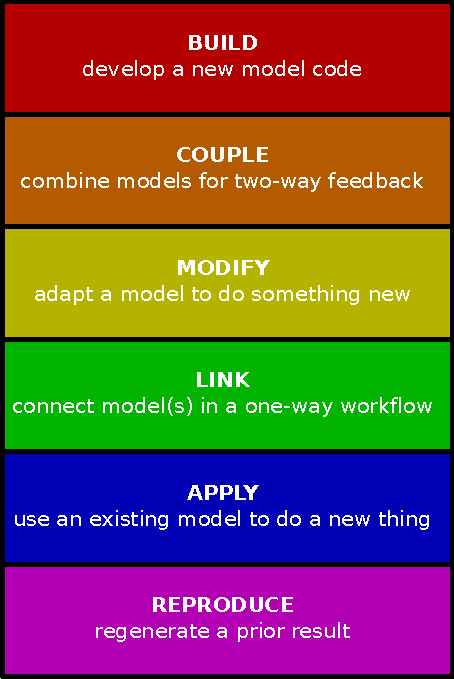
\includegraphics[scale=0.8]{Figures/model_operation_taxonomy.pdf}
\caption{Taxonomy of model operation tasks.}
\label{fig:taxonomy}
\end{figure}


\subsection{Reproducing}

The most basic operation of a numerical model is to run it with a predefined set of parameters and other inputs. This is often the first step in learning how to use a particular model. The ability to reproduce a model calculation efficiently involves all four of the FAIR principles \citep{wilkinson2016fair}. The user must be able to find and access the right version of the software. The user needs to learn how to execute the model: a task made easier if the program follows an interoperability standard. In order to reproduce the prior calculation, the user must also have access to the particular input and configuration data, and must be able to recreate a compatible execution environment, including whatever dependencies (e.g., libraries) might be needed.

\subsection{Applying}

To use a computational model in a new application, a user needs to understand the theory and algorithms behind it, and that requires good documentation. In addition, operating the model involves obtaining and configuring input data, and often executing various pre-processing operations to derive the right kind of inputs. Sometimes it also requires setting up a grid mesh. In some cases, mesh generation is a major undertaking. For example, meshes for 2D storm-surge models such as ADCIRC and 3D regional ocean circulation models such as ROMS could considered major products in their own right.


\subsection{Linking}

Here \textit{linking} means operating a model as part of a sequential, one-way workflow. For example, the workflow might include preprocessing some data, using those data as input to the execution of a model, and using the output from that model as input to another, and/or performing additional operations on the model's output. To link a model in this way requires, among other things, compatibility in data formats (e.g., in files or in data structures that are exchanged in memory). Any incompatibility between the outputs from one step and the inputs to the next means someone has to write code to do the appropriate translation.

\subsection{Modifying}

When an model provides most but not all of the functionality needed for a particular application, the would-be user faces a choice: modify the existing program, or write a new one that fits the purpose. Modifying an existing model program can save a lot of duplication of effort, but only when the model package includes good internal documentation, a modular design, and a structure that allows for modifications and enhancements while preserving the original functionality. A standard interface design can help by providing a familiar structure.

\subsection{Coupling}

Many of the exciting research frontiers in earth and environmental science lie at the seams between systems. Some examples include: rivers and coasts \citep[e.g.,][]{ratliff2018exploring}; tectonics and earth-surface processes \citep[e.g.,][]{roy2016dynamic}; ecosystems, soils, and landscape evolution \citep[e.g.,][]{istanbulluoglu2005vegetation,pelletier2017way,lyons2020speciesevolver}; and human actions and biophysical systems \citep[e.g.,][]{robinson2018modelling}. For these sorts of problem, coupled numerical modeling provides a great way to develop insight and to test hypotheses by comparing models with observations. The complexity of the task of coupling two numerical models depends on the nature of coupling (for example, sequential execution versus coupling via joint matrix inversion) and on the program structure of each. The task becomes much simpler when both models offer a public, standardized interface: a set of callable functions that allow the appropriate exchange of data and mutual execution of algorithms.

\subsection{Building}\label{sec:build}

New ideas stimulate the need for new models. It is a healthy sign of growth when a scientific community produces lots of new models, because it signifies rapid development and exploration of new concepts. Writing a numerical model program from scratch can be a time-consuming exercise that takes time away from other work. Libraries of pre-existing functions and data structures can greatly simplify the task. Most modern programming languages offer libraries to handle basic mathematical operations, but even with these available, model-building can be a major effort in its own right. 

The job becomes easier when the developer can draw on component libraries that provide data structures and algorithms to address common tasks in numerical modeling, such as grid setup and input/output. It becomes easier still when common domain-specific algorithms have been librarized and made available as building blocks with a standard interface \citep[e.g.,][]{brown2014run}. Below we will look at an example of a component library that was designed specifically for building numerical models.



\section{The CSDMS Model Repository: A Platform for Sharing and Archiving Software Resources}

Not all that long ago, making model source code free available was more the exception than common practice. Model developers tended to view their models as trade secrets. If others wanted to use a model, the developer needed to be contacted, and could negotiate to become more involved in the research. Furthermore, fewer easily accessible tools and platforms were available to promote sharing. For example, version control of model source code was something that had to be set up on a server. There were no widely available services like GitHub (established 2008) or SourceForge (established 1999), to enable working with a team on model development, enabling openly sharing models without having to invest in hardware or software.

However, science clearly benefits from openly shared source code. For one, sharing reduces duplication. After all, there is less need to (re)write a model from scratch, once (part of) a model has proven to capture a certain process well. Therefore, sharing of source code accelerates science, as others are on a faster trajectory to learn from and build upon previous model development efforts. Sharing of source code also makes science more robust and trusted. Reproducing computational results requires openly shared source code. Sharing also hardens the code, as people can report bugs and bug fixes. It is therefore encouraging to see a modeling culture shift over the last two decades, in a fashion similar to what has taken place for data \citep[e.g.,][]{hsu2015data}. For good data management, there are now the FAIR principals ---Findability, Accessibility, Interoperability, and Reusability---that have been formulated as guideline to data producers and publishers \citep{wilkinson2016fair}. According to the FAIR principles, each dataset should have a unique digital object identifier (DOI) to get to the data, associated with searchable metadata. By including a formal, broadly applicable representation language, and using open and widely accepted domain-relevant vocabularies and ontologies, data sets become more interoperable. And by providing an abundance of documents that describe datasets and how they can be used, including license information, data become more reusable.

For model source code, version control platforms have been developed, and are now widely used for sharing source code and collaborating in code development. But as the data-FAIR principals indicate, sharing source code by itself is not enough. Therefore, CSDMS implemented the FAIR principles in setting up a model repository for earth surface dynamics. A minimal set of metadata parameters is defined to: describe a model, provide contact information for the model development team, indicate technical details such as operating platform(s) and the software license, describe the model input and output, list its processes and key physical parameters, and indicate limitations. This minimal set of metadata includes a link to the actual source code, which needs to be either made available 24/7 through a personal web repository, or through the CSDMS community repository. All model metadata stored on the CSDMS web server, as well as the actual source code (when stored in the CSDMS code repository on GitHub) are accessible for machines through web APIs, as emphasized by the FAIR protocols to automatically find and use the data, in addition to supporting access by individuals. DOIs for stable versions of the model source code are generated on request and included with the metadata. Model metadata are enriched by including additional reference information, such a comprehensive bibliography pertaining to a particular model. Following this practice, the CSDMS model repository currently holds over 370 open source models of the community (as of June 2020). The models and tools in the repository span a range of languages, with Python, C, and Fortran being the most popular (Figure~\ref{fig:languages}). The diversity of languages raises a challenge in creating an interoperable framework. We will return to this point, and look at one solution, in Section~\ref{sec:babelizer}.

\begin{figure}[h!]
\centering
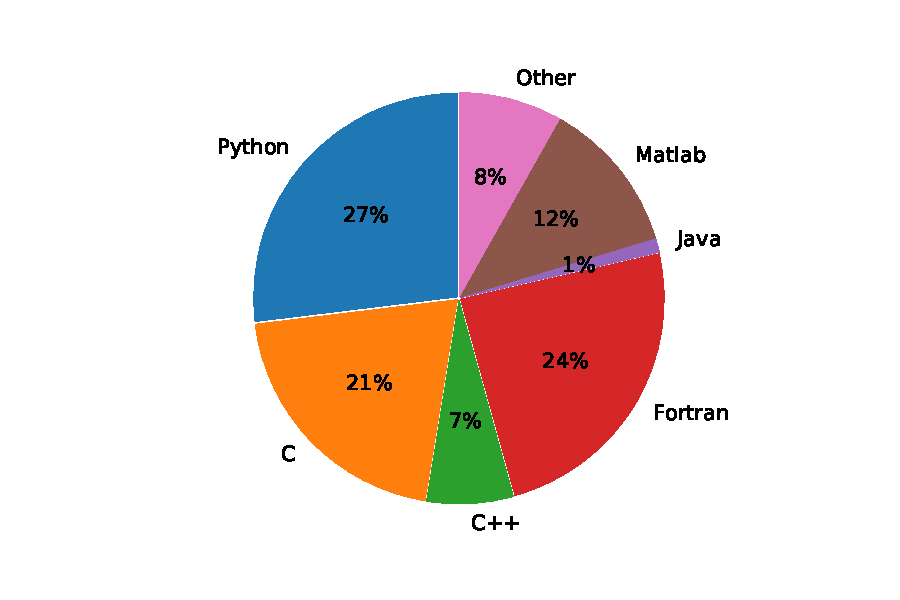
\includegraphics[scale=0.8]{Figures/languages_in_repository.pdf}
\caption{Distribution of different languages used by models and tools in the CSDMS Model Repository (percentages out of 453 total programs; not weighted by program size).}
\label{fig:languages}
\end{figure}


\section{The CSDMS Workbench}
\label{sec:workbench}

The \textbf{CSDMS Workbench} is a suite of tools, standards, documents, and resources that collectively provide a modular environment for model execution, analysis, and model-data integration. The Workbench comprises five main elements \ref{fig:workbench}: 
\begin{enumerate}
    \item The Basic Model Interface (BMI): an interface standard that simplifies model execution and coupling \citep{hutton2020basic}.
    \item Babelizer: a language interoperability tool that adds a Python interface to BMI-enabled model programs written in various other languages.
    \item PyMT: a Python-language execution and model-coupling environment, which includes utilities for grid mapping and other operations.
    \item Data Components: small Python-language modules that use the BMI to fetch data from particular data sets.
    \item Landlab: a component-based Python library for model building and sharing of interoperable components \citep{hobley2017creative,barnhart2020short}.
\end{enumerate}

\subsection{The Basic Model Interface (BMI) Standard}

%- standardization: BMI

%(note: this isn't meant to be a substitute for the BMI papers; it's just a relatively short summary, probably with a table or figure, plus a figure illustrating an application in the literature or underway, e.g., Hoch et al. (2017) and/or PRMS)

% Outline:
% 1. Intro to idea of BMI (use Greg's intro to BMI docs
% 2. Description of BMI methods
%   a. Include table
%   b. Include sample code
% 3. Example of BMI use in research (I like Greg's suggestion of Hoch paper)
%   a. Include figure

When you sit in the driver's seat of an unfamiliar car,
you're presented with a familiar sight:
whatever the make or model,
we take it for granted that a car provides
a steering wheel, brake pedal, and speedometer.
%along with other controls and readouts
%that are common to essentially all cars on the planet.
Although we don't usually think of it this way,
drivers across the globe benefit
from a standard interface---a set of control mechanisms and information displays
that have %basically
essentially the same design
regardless of whether the car
is a tiny electric two-seater or a giant stretch limousine.
This standard interface makes operating a car much easier
than if each vehicle presented a radically different interface.
Imagine a world where switching from a sports car to a pickup truck
required months of study and practice!

We believe %that
numerical models should offer a similar standardization.
To this end, CSDMS
developed the Basic Model Interface (BMI) \citep{peckham2013component,hutton2020bmi}.
%a set of standard control and query functions for models.
In software engineering,
an interface is a named set of functions
with prescribed arguments and return values.
The BMI provides a standard set of functions
for querying and controlling a model.
Just as with a car,
when a model is equipped with a BMI,
it becomes easier to use
because its control functions are now the same as every other model with a BMI.
%once you've seen one BMI, you've seen them all.
Further, because BMI includes variable exchange functions,
a model with a BMI can be coupled with other models that expose a BMI.
Table \ref{tab:bmi} lists the individual functions
that comprise the Basic Model Interface,
along with a brief description of each.
The table shows the current version of BMI, version 2.0,
which represents a collection of improvements to the original specification,
especially in the representation of model grids \citep{hutton2020bmi}.

\begin{table}[htbp]
    \Small
    \topcaption{Listing and description of Basic Model Interface (BMI) functions.}
    \begin{tabular}{ll}
        \hline
        Function Name &
        Description \\
        \hline\hline
        
        \verb|initialize| & Perform startup tasks for the model. \\
        \verb|update| & Advance model state by one time step. \\
        \verb|update_until| & Advance model state until the given time. \\
        \verb|finalize| & Perform tear-down tasks for the model. \\
        \verb|get_component_name| & Name of the model. \\
        \verb|get_input_item_count| & Count of a model’s input variables. \\
        \verb|get_output_item_count| & Count of a model’s output variables. \\
        \verb|get_input_var_names| & List of a model’s input variables. \\
        \verb|get_output_var_names| & List of a model’s output variables. \\
        \verb|get_var_grid| & Get the grid identifier for a variable. \\
        \verb|get_var_type| & Get the data type of a variable. \\
        \verb|get_var_units| & Get the units of a variable. \\
        \verb|get_var_itemsize| & Get the size (in bytes) of one element of a variable. \\
        \verb|get_var_nbytes| & Get the total size (in bytes) of a variable. \\
        \verb|get_var_location| & Get the grid element type of a variable. \\
        \verb|get_current_time| & Current time of the model. \\
        \verb|get_start_time| & Start time of the model. \\
        \verb|get_end_time| & End time of the model. \\
        \verb|get_time_units| & Time units used in the model. \\
        \verb|get_time_step| & Time step used in the model. \\
        \verb|get_value| & Get a copy of values of a given variable. \\
        \verb|get_value_ptr| & Get a reference to the values of a given variable. \\
        \verb|get_value_at_indices| & Get variable values at specific locations. \\
        \verb|set_value| & Set the values of a given variable. \\
        \verb|set_value_at_indices| & Set the values of a variable at specific locations. \\
        \verb|get_grid_rank| & Get the number of dimensions of a computational grid. \\
        \verb|get_grid_size| & Get the total number of elements of a computational grid. \\
        \verb|get_grid_type| & Get the grid type as a string. \\
        \verb|get_grid_shape| & Get the dimensions of a computational grid. \\
        \verb|get_grid_spacing| & Get the spacing between grid nodes. \\
        \verb|get_grid_origin| & Get the origin of a grid. \\
        \verb|get_grid_x| & Get the locations of a grid’s nodes in dimension 1. \\
        \verb|get_grid_y| & Get the locations of a grid’s nodes in dimension 2. \\
        \verb|get_grid_z| & Get the locations of a grid’s nodes in dimension 3. \\
        \verb|get_grid_node_count| & Get the number of nodes in the grid. \\
        \verb|get_grid_edge_count| & Get the number of edges in the grid. \\
        \verb|get_grid_face_count| & Get the number of faces in the grid. \\
        \verb|get_grid_edge_nodes| & Get the edge-node connectivity. \\
        \verb|get_grid_face_edges| & Get the face-edge connectivity. \\
        \verb|get_grid_face_nodes| & Get the face-node connectivity. \\
        \verb|get_grid_nodes_per_face| & Get the number of nodes for each face. \\
    \hline
   \end{tabular}
   \label{tab:bmi}
\end{table}

While a BMI can be written for any language,
CSDMS currently supports four languages: C, C++, Fortran, and Python.
A simple example of using a BMI written in Fortran
is shown in Listing~\ref{listing:bmi_code} below.
%
% minted is super cool, nicer than just verbatim -MP
\begin{listing}[ht]
\topcaption{Example Fortran BMI code.}
\begin{minted}{fortran}
  type (bmi_prms_surface) :: model
  character (len=*) :: config_file
  integer :: status
  double precision :: now, end_time

  status = model%initialize(config_file)
  status = model%get_current_time(now)
  status = model%get_end_time(end_time)
  do while (now < end_time)
     status = model%update()
     status = model%get_current_time(now)
  end do
  status = model%finalize()
\end{minted}
\label{listing:bmi_code}
\end{listing}
%
The model shown in this example
is the surface water component of the Precipitation Runoff Modeling System (PRMS),
developed by the U.S. Geological Survey \citep{leavesley1984precipitation}.
In the example,
the model is initialized from its native configuration file,
then stepped forward in time until it reaches its stop time,
whereupon any resources it uses are deallocated.
Note that only BMI function calls are used to drive the model;
no knowledge of the underlying native calls to control PRMS are needed.

\cite{hoch2019evaluating} provide a current research example of using BMI. 
In their study,
they coupled a hydrologic model, PCR-GLOBWB,
with a pair of hydrodynamic models, CaMa-Flood and LISFLOOD-FP,
through BMI.
They observed (see Figure~\ref{fig:hoch_2019_fig6}) that a coupled model system
enhanced the accuracy of peak discharge simulations.
%and improved representation of observed flood extent in flood maps
%(Figure 7 from their paper).
%
\begin{figure}[h!]
\centering
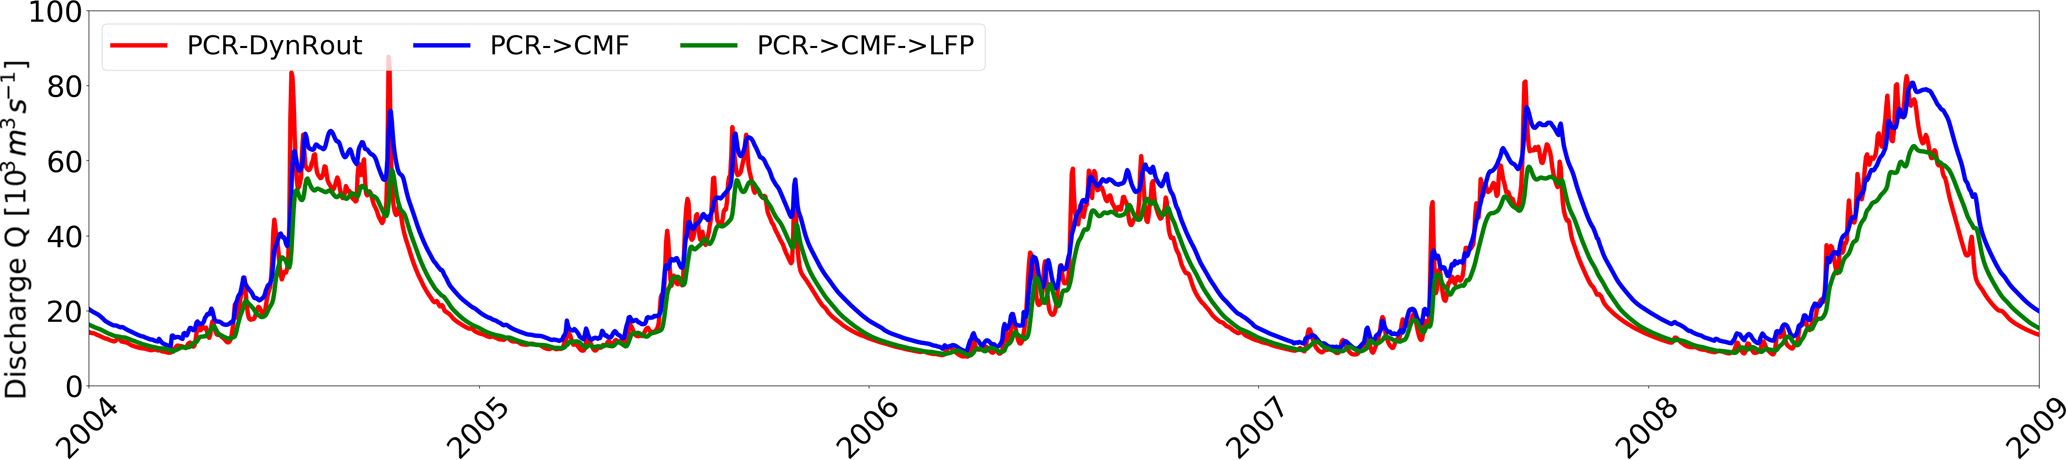
\includegraphics[scale=0.8]{Figures/nhess-19-1723-2019-f06.png}
\caption{Simulated discharge at a river monitoring station from coupled hydrologic and hydrodynamic models. (Reproduced from Figure 6 from \citet{hoch2019evaluating}.)}
\label{fig:hoch_2019_fig6}
\end{figure}
%
\citeauthor{hoch2019evaluating} conclude
that ``Results confirm that model coupling can indeed be a viable way forward towards more integrated flood simulations. However, results also suggest that the accuracy of coupled models still largely depends on the model forcing.''

\subsection{Language Interoperability: The Babelizer}
\label{sec:babelizer}

refer to Figure~\ref{fig:languages} somewhere in this section

- need a lingua franca; here, Python because of its popularity, num/sci libraries, and high-level interpreted nature

- babelizer: tools and procedures to take BMI'd code in C, C++, F, (Julia??) and convert to Python-callable module



- notion that the BMI specification makes it relatively straightforward to add a language (or should this go under BMI?)

\begin{figure}[h!]
\centering
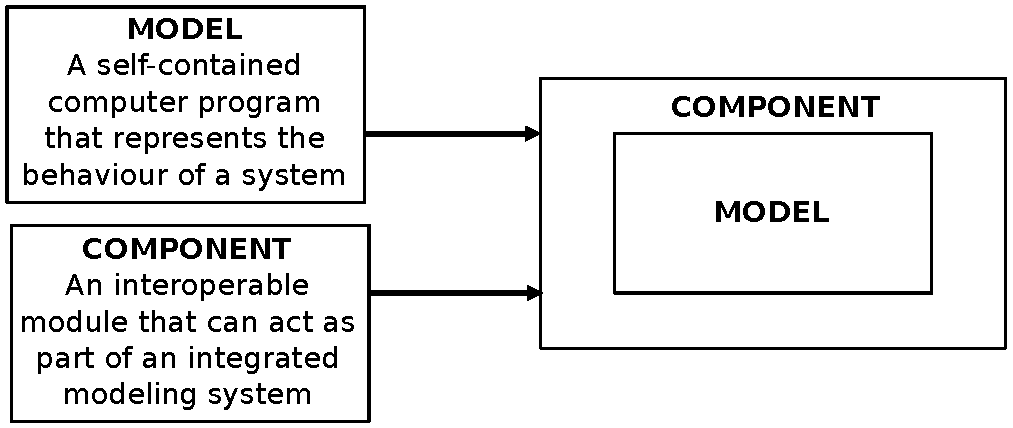
\includegraphics[scale=0.5]{Figures/model_to_component.pdf}
\caption{When a numerical model program is `wrapped' with a standard interface and compiled as an importable module, it becomes an interoperable \textit{component}.}
\label{fig:component}
\end{figure}


\subsection{Execution and Coupling Framework: pymt}

-- what pymt is

- do we also include mention, maybe pictures, of its predecessors?

-- table of components, including domain of each

- examples: Ratliff river-delta picture; Wang permafrost picture

\subsection{Data Components}

Researchers rarely use numerical models in isolation. Working with models nearly always includes working with data sets too: both the data that go into a model as input, and the output data that the model produces (Table~\ref{tab:taxonomy}). Productivity suffers when these data sets are cumbersome to access and use. Just as model interface standards like BMI make it easier to work with numerical models, standardized methods for data access and retrieval can ease the burden of working with data. To that end, CSDMS has developed a programmatic approach that uses the BMI for data retrieval and access. Functions such as \texttt{initialize()} retrieve and open a data set, and \texttt{get\_value()} fetches particular data items or subsets. A program that uses the BMI to access items from a particular data set is known as a \textit{Data Component}. Using the same interface for model and data operation makes it easier to swap models and data sets; for example, one might compare use of model-calculated versus measured wave heights in a simulation of coastal sediment transport. [TODO: IF WE GET FAR ENOUGH, ADD MENTION OF COMPATIBILITY OF DATA COMPONENTS WITH LANGUAGE-SPECIFIC DATA LIBRARIES LIKE XARRAY]

The data components are designed to provide a consistent way to access various types of datasets (e.g., time series, raster grid, and multidimensional space-time data) and subsets of them without needing to know the original file formats. Each data component effectively `wraps' a dataset with a BMI. Data components can easily interact with BMI-enabled numerical models in the pymt modeling framework, or other similar frameworks.

One example is the National Water Model (NWM) data component. This data component can access and subset the forecasted streamflow time series generated by the NWM hydrologic modelling framework. Figure \ref{fig:data_component1} shows an example of how the NWM data component can be used to get the streamflow data at a river channel for a flooding event. Figure \ref{fig:data_component2} shows the corresponding time series plot. This data component includes a set of standard control and query functions (e.g.,  \texttt{initialize()} , \texttt{update()}). These standard methods make the dataset easier to couple with BMI-enabled numerical models  without needing to know the time-series file format.

\begin{figure}[h!]
\centering
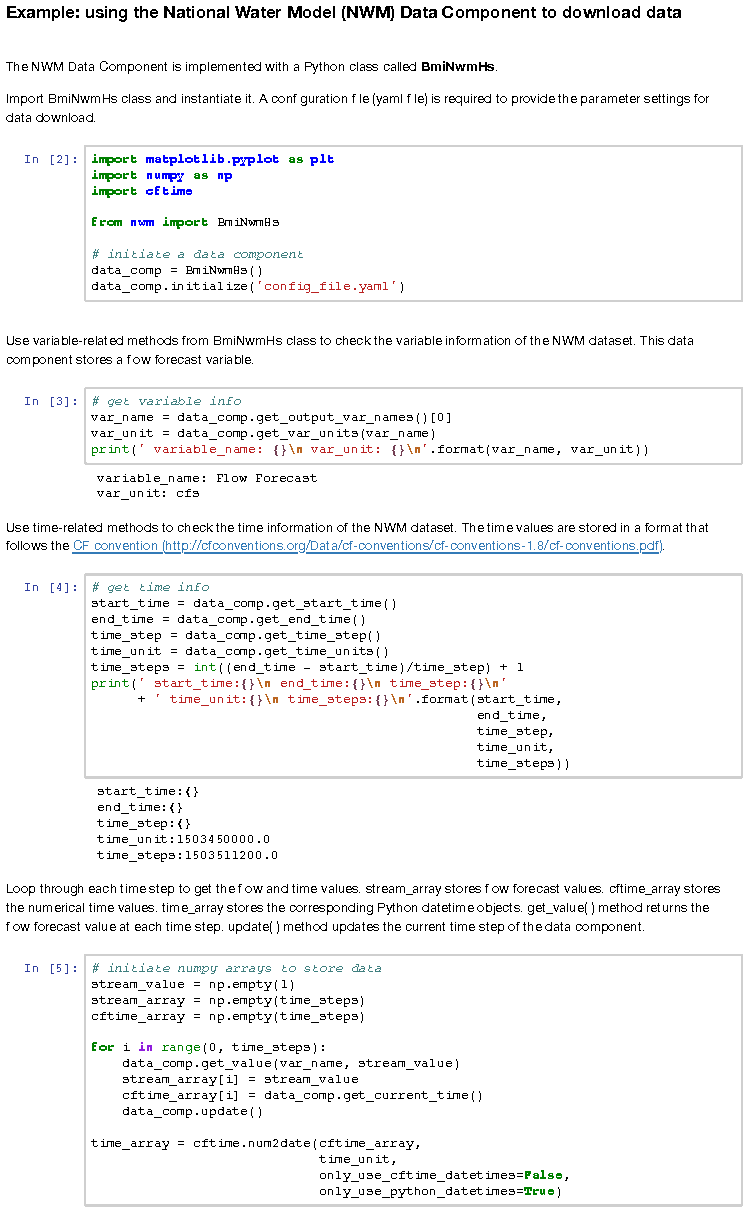
\includegraphics[scale=0.8]{Figures/nwm_example_notebook.pdf}
\caption{Screenshot of a JupyterNotebook demonstrating how to use nwm data component to access and subset streamflow dataset. }
\label{fig:data_component1}
\end{figure}

\begin{figure}[h!]
\centering
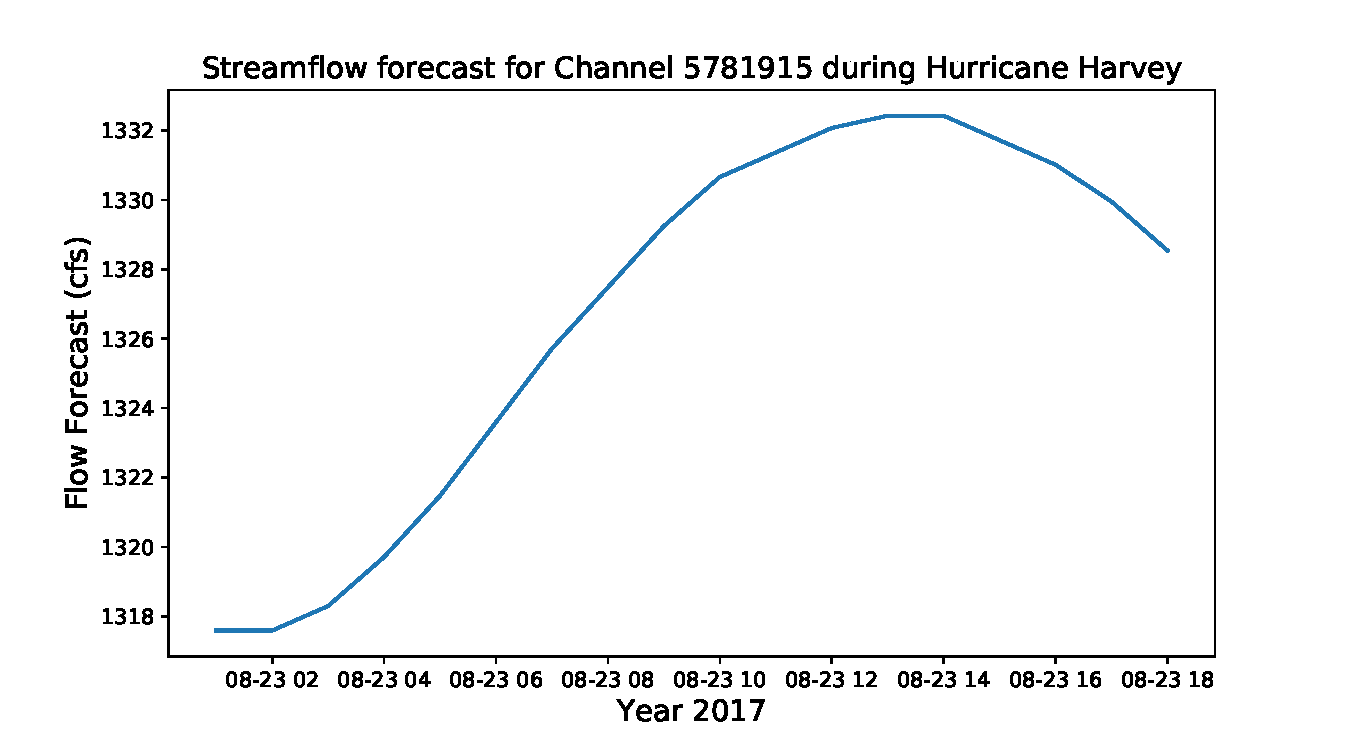
\includegraphics[scale=0.5]{Figures/nwm_hydrograph.pdf}
\caption{Time series plot for the accessed streamflow dataset. }
\label{fig:data_component2}
\end{figure}


\subsection{Creating new models: Landlab}

Landlab is a Python-language library designed to support the creation, combination, and re-use of 2-D models \citep{hobley2017creative, barnhart2020short}. For the moment, let's presume that a model developer has identified input and output parameters, model state variables, and the governing equations and/or model rules. We might then synthesize the tasks of building the model (Section~\ref{sec:build}) into two types: (a) creating required data structures, and (b) implementing governing equations that act on those data structures. For example, most models need to represent the computational domain, including information (such as the current value of state variables) across the domain, and adjacency information describing how the different parts of the domain are connected to one another. This division is clearly simplistic, and neglects many intricacies, yet it captures the fundamental activities of model building. 

Landlab provides re-usable software infrastructure that addresses the most common needs for our two model building tasks. For grid-based data structures, Landlab provides a \textit{grid} object to represent the computational domain and store \textit{fields} of state variables. Landlab provides multiple grid types through a similar interface (e.g., regular raster, network, regular hexagon, irregular). For all grid types, the adjacency information and access to fields follows the same interface---making it nearly trivial for a model to work on multiple grid types. 

To address the second model-building task, Landlab provides two capabilities. First is a set of numerical utilities that support common needs. These include, for example, the ability to calculate differences, fluxes, and divergences of values stored at fields. Second is a library of \textit{Components}. In general, each Landlab component simulates a single process (e.g., stream power erosion, linear diffusion). Components are implemented as Python classes, and are derived from a common base class that enforces a minimum amount of model metadata for each model and defines common attributes. If a model, or part of model is implemented within Landlab as a Component, the model author need only write the code to instantiate a model, and to run it forward in time.

The Component base class was designed to expose a BMI such that conversion of Landlab Components to pymt components is trivial. 
\todo[inline,color=yellow]{KRB: I think it would be best if Eric finished this section}

Despite the name, Landlab is not restricted to terrestrial processes. Its component collection includes, for example, coastal and marine components for processes such as tidal circulation and deltaic sedimentation. More generally, its design is amenable to a wide variety of 2D grid-based numerical models and cellular automata applications beyond the earth and environmental sciences. Landlab can be used, for example, to construct integrated source-to-sink models that treat the full geologic cycle, tracking sediment from its creation on land to its deposition in marine basins (Figure~\ref{fig:riftisland}).

\begin{figure*}
\includegraphics[width=14cm]{Figures/LS-Overview.png}
\caption{Illustration of HyLands model component. \textbf{a.} Time slices showing evolution of the landscape to steady state, without landsliding. The blue line represents the location of the river plotted in subplot (e). \textbf{b.} Same as (a), with landsliding. \textbf{c.} Sediment accumulation and the formation of alluvial fans. \textbf{d.} Landslide activity during the depicted time step. Red colors represent the logarithm of the landslide erosion, blue colors represent deposition. (e.) Shows the topographic and bedrock elevation (red and black line respectively) and the sediment thickness (orange line). The sediment flux is plotted against the right-hand y-axis (blue line). Note that, during landsliding, both pure landslide dams arise (red bumps on the profile) as well as irregularities in the bedrock profile (grey bumps). The latter originate from the river being redirected after landsliding, forming epigenetic gorges.}
\label{fig:landslides}
\end{figure*}

\begin{figure}
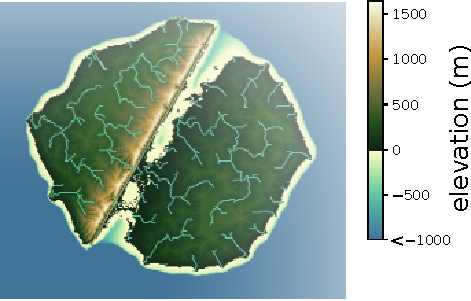
\includegraphics[width=10cm]{Figures/rift_island.pdf}
\caption{Snapshot from an integrated numerical model of landscape and sedimentary basin evolution. Domain size is 250 by 250 km. Simulation shows a hypothetical micro-continent with an active NNE-oriented extensional fault. Sea level varies stochastically; this particular snapshot captures a relative lowstand. Model was constructed using Landlab components for flow routing (\textit{FlowAccumulator, FlowDirectorSteepest, LakeMapperBarnes}), fluvial processes (\textit{ErosionDeposition}), marine sediment transport (\textit{SimpleSubmarineDiffuser}), and extensional faulting (\textit{KinematicExtender}). Colormap designed by \citet{thyng2016true}.}
\label{fig:riftisland}
\end{figure}

The design of Landlab supports a variety of usage styles. Interested users and/or developers may use Landlab to create models as Components, or as scripts that combine components. Alternatively, Landlab can be used to build stand-alone packages packages such as \texttt{terrainbento} \citep{barnhart2019terrainbento}, which combine Landlab Components into a predefined set of models.

% GREGS NOTES:
% - relatively brief summary, pointing toward Hobley and Barnhart papers

% - include LL components as lighter-weight version of BMI components (because it's explicitly Python based, so don't need the extra overhead of BMI)

% - include mention of how a LL component gets converted to a pymt component

\subsection{Example of a new model component: Landslides}
  
The modular infrastructure of Landlab enables the development of numerical tools in a quick and efficient manner. An example of a recently developed Landlab component is HyLands: a ``hybrid'' landscape evolution component that simulates mass wasting and sediment redistribution on hillslopes. The model was originally developed within proprietary software \citep{Campforts2020} and will now be available as an open source tool for the broader community. The grid engine and a wide variety of numerical tools available within the Landlab library enabled efficient implementation and provides capabilities for online coupling with other, existing Landlab components. An example is the Stream Power with Alluvium Conservation and Entrainment (SPACE) component which has been developed to simulate fluvial sediment transport and incision \citep{shobe2017space} and is showcased here as an example of model coupling in HyLands. 

The integration capabilities of Landlab, where new and existing components can be combined in a straightforward way, opens up new possibilities for applied environmental engineering and fundamental scientific research. For HyLands in specific, the coupling of a deep-seated landslide algorithm with a sediment routing system will (i) help on a more applied level to explore the impact of future changes in storm frequency on landslide occurrence and sediment dynamics  \cite{Fan2019} and (ii) on a more fundamental level to facilitate the investigation of the interaction between landslides and sediment dynamics over geological timescales. The latter is illustrated in figure \ref{fig:landslides} where we use the Landlab software to simulate the impact of uplifting terrain on the formation of alluvial fans. Simulations are executed with and without landslide activity (figure \ref{fig:landslides}.a vs. figure \ref{fig:landslides}.b). Resulting magnitude frequency and area volume relationships for the simulated landslides are shown in figures \ref{fig:MF-landslides}. The evolution of the alluvial fans is further visualised in the movies listed in Table \ref{tab:LS-movies}. For details regarding the algorithms and physics supporting the HyLands component, see \citep{Campforts2020}. 

\begin{figure*}
\includegraphics[width=14cm]{Figures/LS-Overview.png}
\caption{Illustration of HyLands model component. \textbf{a.} Time slices showing evolution of the landscape to steady state, without landsliding. The blue line represents the location of the river plotted in subplot (e). \textbf{b.} Same as (a), with landsliding. \textbf{c.} Sediment accumulation and the formation of alluvial fans. \textbf{d.} Landslide activity during the depicted time step. Red colors represent the logarithm of the landslide erosion, blue colors represent deposition. (e.) Shows the topographic and bedrock elevation (red and black line respectively) and the sediment thickness (orange line). The sediment flux is plotted against the right-hand y-axis (blue line). Note that, during landsliding, both pure landslide dams arise (red bumps on the profile) as well as irregularities in the bedrock profile (grey bumps). The latter originate from the river being redirected after landsliding, forming epigenetic gorges.}
\label{fig:landslides}
\end{figure*}

\begin{figure*}[t]
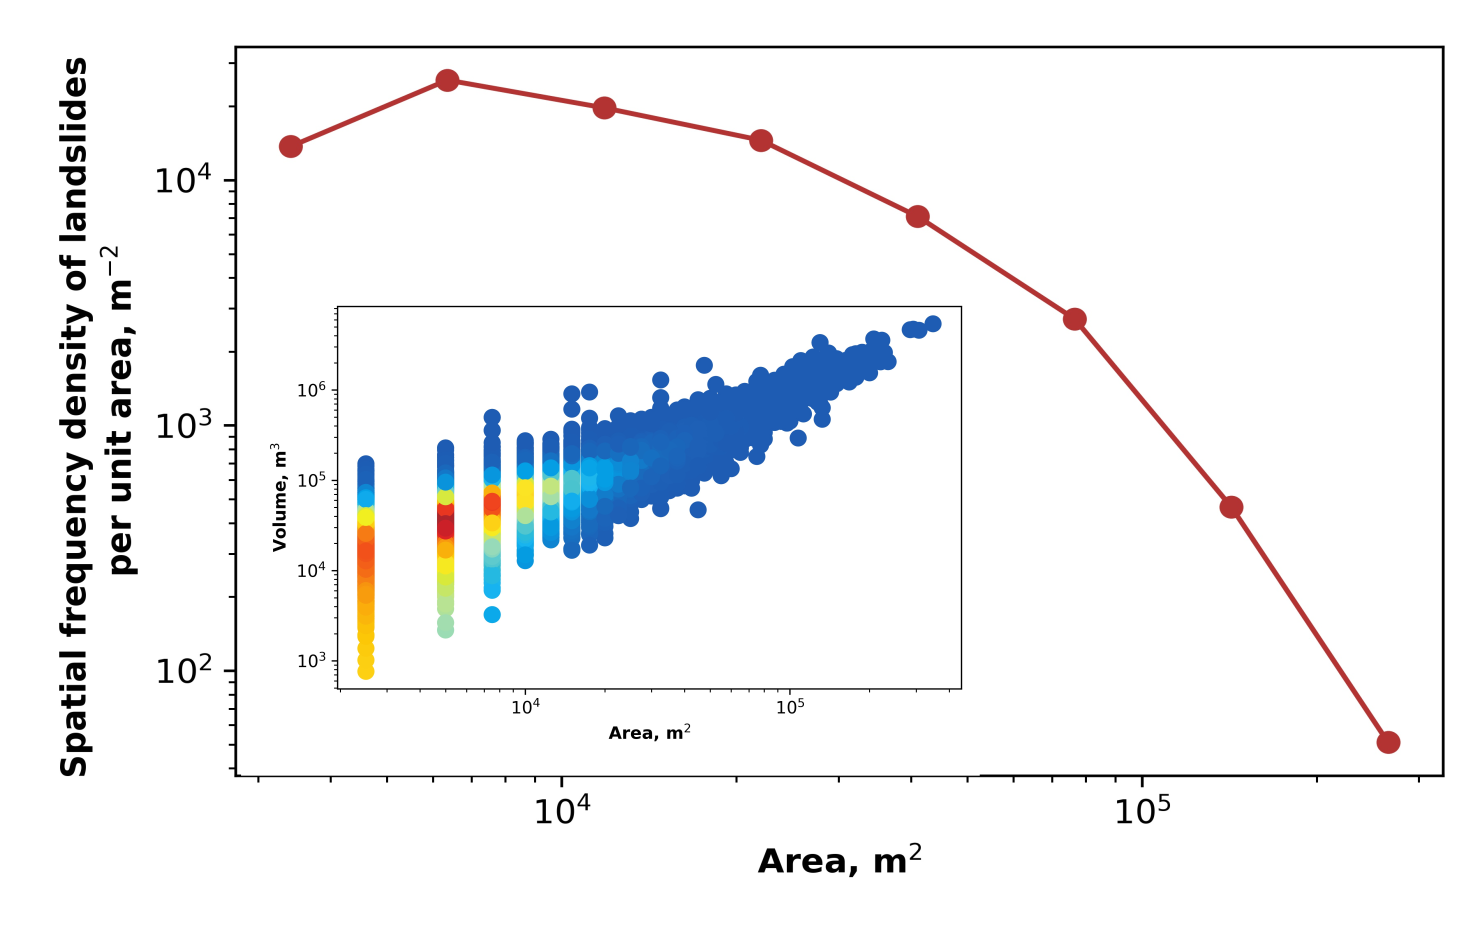
\includegraphics[width=10cm]{Figures/LS-Mag-Freq.png}
\caption{(\textbf{a}) Magnitude-frequency relationship of the landslides simulated with Landlab-HyLands (red dots) and illustrated in figure \ref{fig:landslides}. (\textbf{Inset}) Scatter density plot showing the simulated Area-Volume relationship.}
\label{fig:MF-landslides}
\end{figure*}

\begin{table}[htbp]
    \Small
    \topcaption{Simulation movies created with Landlab-HyLands}
    \begin{tabular}{lll}
        \hline
        Scenario & Description & Link\\
        \hline\hline
        \verb|No landslides| &\verb|topography | & \url{https://youtu.be/c5d7T8eehxw} \\
        \verb|| &\verb|location of longest river|& \url{https://youtu.be/GqokukWi9cs} \\
        \verb|| &\verb|river profile |& \url{https://youtu.be/A_JZ9POfJ54} \\
        \verb|| &\verb|sediment thickness |& \url{https://youtu.be/t0_tel5fhbM} \\
        
        \verb|Landslides| &\verb|topography | & \url{https://youtu.be/1K_ceKYt9Nw} \\
        \verb|| &\verb|location of longest river|& \url{https://youtu.be/YkmbUTN7zlI} \\
        \verb|| &\verb|river profile |& \url{https://youtu.be/jyWgKTcMe74} \\
        \verb|| &\verb|sediment thickness |& \url{https://youtu.be/rwEBqGtHZs0} \\
        \verb|| &\verb|landslide erosion and deposition |& \url{https://youtu.be/_xoSm7p4ZxI} \\
    \hline
   \end{tabular}
   \label{tab:LS-movies}
\end{table} 

\subsection{OPTIONAL: Model analysis: Dakota and Dakotathon}

- do we want to include this?

\section{Software Development Practices}

- VC

- testing and CI

- creating the documentation (and how much is enough?)
   - API documentation vs examples (typically notebooks)

- collaboration: issues and PRs


\section{Community Engagement}
\label{sec:community}

One of CSDMS' major activities has been the creation of a thriving community around earth-surface dynamics modeling \citep{overeem2013strategies}. As of 2020, over 1,900 members, representing 552 institutions (144 US academic) and 71 countries, had joined the community.  CSDMS is, by design, a broad and deep coalition of members from disciplines reflected by the five Working Groups and seven Focus Research Groups (Figure~\ref{fig:groups}).  From its inception, CSDMS has encouraged trans-disciplinarity by providing opportunities such as annual meetings, workshops, hackathons, and training events for domain scientists to interact with colleagues from other earth and social science disciplines.  These connections are essential for knowledge exchange among community efforts and allow for wider penetration of new technology and ideas. Cross-pollination of ideas from these events and other community-member interactions have lead to a variety of independently funded research projects. CSDMS has played a key role in shifting the paradigm for open code sharing in the earth surface processes by facilitating resource sharing through model, data, and education repositories on the CSDMS web portal.  CSDMS also offers a variety of services to community processes and the geoscience subdiscipline of interest.  But along with their disciplinary expertise, however, they also need a strong foundation in programming, advanced computing skills and data analytics skills \citep{atkins2011national}.
Traditional Earth science education does not usually equip students with skills to use modern cyberinfrastructure and computing resources efficiently, or to become model developers \citep{campbell2013taking}. The Earth Surface Processes (ESP) community critically needs a platform to teach modern programming practices and high-performance computing methods to develop innovative models that can be used to understand and predict how the earth’s surface responds to environmental change and human influence.
The practice of modeling lies at the core of predictive ESP sciences, and educators should engage students in building, testing, and applying models \citep{hestenes1996modeling,manduca2008making}, but we found from a review of course catalogs that in practice the undergraduate curricula of more traditional disciplinary focused departments do not include this component \citep{campbell2013taking}. This issue is not entirely unique to ESP sciences. The geosciences today are intensively quantitative, and there is an urgent need for a workforce with strong STEM skills \citep{national2012discipline}. The United States' National Science Foundation (NSF) recognizes as one of its `10 Big Ideas' that pathways are needed for educators to create a 21st-century workforce capable of effectively dealing with data [ED Office of Educational Technology, 2017]. Moreover, an agile STEM workforce is considered a national priority \citep{atkins2011national}. Realizing this, CSDMS provides hands-on training opportunities during meetings. Some efforts are meant to built foundation---for example, by teaching graduate students skills in best programming practices and version controls in day-long short courses. Other outreach efforts consist of short clinics, targeted to give potential users of cyberinfrastructure an active feel for certain models or modeling techniques, or to provide an update to experts on new developments.  More extensive separately organized hackathons bring together small science teams to work on solutions for more specific outstanding research problems.  For the first time in 2020, an immersive Earth Surface Processes Summer Institute is being organized online for a large group of students and early career scientists, focused solely on capacity building for East Surface Processes modeling.

\begin{figure}[h!]
\centering
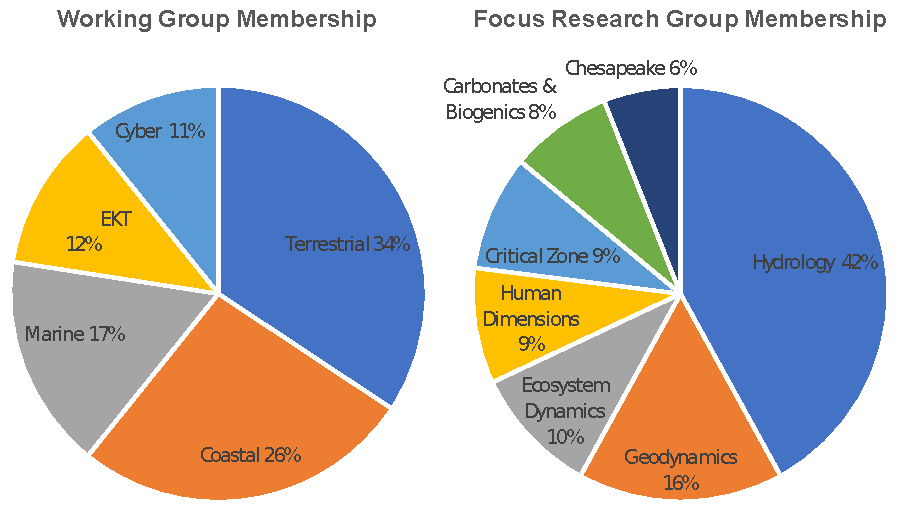
\includegraphics[scale=0.9]{Figures/working_and_focus_groups.pdf}
\caption{CSDMS Working Groups and Focus Research Groups.}
\label{fig:groups}
\end{figure}


\section{Discussion}
\label{sec:discussion}

In May 2020, the US National Science Foundation released a special report, prepared by the National Academy, on research opportunities in the earth sciences. The report highlighted three unique types of research infrastructure: instrumentation, human infrastructure, and cyberinfrastructure. The recognition of cyberinfrastructure as a distinct form of research infrastructure signifies the critical role that computing now plays in the earth and environmental sciences. Environmental modelling, and the software and culture-of-practice that supports it, constitutes a key part of that cyberinfrastructure. In other words, research software is infrastructure, and deserving of the same care and attention as a laboratory or field station.

The research enterprise benefits when modeling  software and tools are shared, coordinated, and interoperable, such that the six model operation tasks listed in Table~\ref{tab:taxonomy} are simplified. For the earth surface sciences, the CSDMS Model Repository provides a community platform for finding and sharing model codes and related tools. In addition to acting as a valuable community resource, the Repository provides a solution to the growing mandate from journals and funding agencies to make research software openly available. The provision of standardized metadata and bibliographic information helps those who are looking for models to compare and evaluate the alternatives.

Simply providing source code and metadata is not enough, however. In order for earth and environmental models to function as community resources, they must be usable. One of the key dimensions of usability is interoperability. The BMI standard promotes interoperability by reducing the learning curve for executing and querying models, and by greatly simplifying the process of linking (one way) or coupling (two way) models. A model program equipped with a BMI becomes an interoperable, standardized component: an element of a system, rather than an idiosyncratic stand-alone product. One of the key abilities offered by a BMI-enabled model is run-time control, query, and modification. Because BMI supports step-wise execution, a user can effectively pause a model in mid-run to inspect its state variables, and modify parameters or data. This capability allows sequential coupling of models using simple scripts. The ability to query and modify values also enables tight coupling. For example, if a collection of component models are treated as representing individual terms in a governing equation, a coupling script could be used to query each component's derivatives, construct a matrix, solve it, and then pass the updated state variables back to the individual components.

One advantage of BMI is that it is language agnostic, and can in principle be implemented in nearly any programming language. It can, for example, accommodate legacy codes written in Fortran. The disadvantage of language flexibility is that BMI addresses the least common denominator, and therefore does not take advantage of the more advanced features available in some languages, such as object-oriented capabilities. To some extent this disadvantage can be addressed by building more specialized, language-specific interfaces in parallel with a BMI. For example, Landlab components, which are implemented as classes, use a lightweight, Python-specific interface that takes advantage of that language's object-oriented capabilities, advanced data types, and parameter-passing syntax. At the same time, Landlab also includes functionality to translate any of its components into a standard BMI component, so they can be integrated with components written in other languages.

The flexibility that BMI offers has led to its adoption in a variety of different applications, including US Geological Survey rainfall-runoff models \ref{}, hydrodynamic modeling (including flagship models developed by Deltares and the Netherlands eScience Center) \ref{}, delta and coastline evolution modeling \ref{ratliff2018}, and modeling of methane emissions \ref{fox2020agent}, to name a few. One disadvantage of a standard interface like BMI is the extra up-front investment in program development. Researchers may not perceive value in adding a standard interface to a legacy code, or writing it into a new code. However, our experience is that this effort usually more than pays for itself over the duration of a project. Code written to a standard like BMI tends to be more modular and therefore easier to maintain. Existing templates for common languages in the earth and environmental sciences make the process of providing a BMI to a new program is relatively painless: just a matter of filling in a set of pre-defined function names and signatures \citep{hutton2020basic}. Adding a BMI to an existing legacy model can be a bit more involved, depending on how the program code is structured, because it often requires some degree of refactoring. Even in that case, we find that adding a BMI to a legacy model often makes that code more understandable and adaptable.

The variety of different programming languages used in the earth and environmental sciences community presents a barrier to interoperability. The majority of models and tools in the CSDMS Repository are written in C, C++, Fortran, Python, and Matlab \ref{}[ADD FIGURE]. Other languages used in CSDMS constituent communities include R (especially in ecosystem dynamics) and NetLogo's java-based scripting language (for agent-based modeling). Crossing the language barrier requires language-bridging tools. Translating all of the existing code into a single, common language would be impractical, even if the community could agree on which language to use. A more effective solution is to \textit{librarize} models and tools \citep{brown2014run} as components that can be accessed and executing through a high-level scripting language. In CSDMS' case, the Babelizer tool provides this capability for codes written in C, C++, and Fortran, using Python as the high-level linga franca.

Librarization can be applied to data sets too. The CSDMS Workbench accomplishes this with Data Components that provide function-call access to various data sets. Using the BMI syntax for data access removes the need to worry about data formats, and makes it easier to swap between data sets and models (for example, data versus model of ocean-wave properties) as components in a linked system. In this case, the BMI does not replace the more sophisticated data-access capabilities of a language-specific library like xarray, but it has the advantage of providing a consistent interface across multiple languages.

For building and modifying numerical models, the CSDMS Workbench provides Landlab as a Python-specific solution for 2D, grid-based applications. Experience with Landlab since its introduction has shown that a library of model `building blocks' can greatly reduce the barriers to the software side of model creation. One indicator of the success of this approach is the growing number of  Landlab-built models created by doctoral students as part of a larger body of dissertation research \citep[e.g.,][]{adams2017landlab,gray2017off,shobe2017space,lai2018modeled,langston2018developing,schmid2018effect,strauch2018hydroclimatological,glade2019canyon,reitman2019offset,carriere2020impact,litwin2020groundwaterdupuitpercolator}. The ability to assemble models out of reusable `process components' allows for rapid construction of complete, multi-element models. One example of the value of rapid model assembly is a recent  comparative testing and calibration study of long-term landform evolution models \citep{barnhart2020inverting1,barnhart2020inverting2}. The study authors used Landlab to develop a Python package for multi-model analysis of drainage basin evolution \citep{barnhart2019terrainbento}. The package allowed for the exploration and testing of 37 mathematically distinct models, as alternative hypotheses. This example illustrates how flexible, component-based modeling software promotes hypothesis testing. 

Experience with BMI, pymt, and Landlab highlights the critical importance of documentation, consistent with the findings of \citet{lawrence2015science}. Tutorial examples in particular provide a starting point that users can build on. Embedding tutorials in Jupyter Notebooks provides an effective way to combine descriptive text, program code, plots, and formatted mathematics. For reference-level documentation, document generator tools like Sphinx and doxygen translate internal documentation (comment blocks inside source code) into nicely formatted, web-accessible reference material.

A successful community cyberinfrastructure for numerical modeling requires more than just technology. It also takes community building and coordination. In the case of CSDMS, the community centers around common interest in a broader theme (earth-surface processes) and a common approach (modeling). Activities such as meetings, workshops, hackathons, and webinars can help draw attention new of tools and methods, provide education in their use, and contribute to building a culture of resource sharing.

One of the biggest challenges to a fully functional community software ecosystem in earth and environmental modeling is the paucity of technical training. As noted earlier, many geoscientists are self-taught programmers, and generally unaware of practices and tools that would make their work more efficient and sustainable. CSDMS and other community facilities have had some success in addressing this need with workshops, webinars, and summer schools, but there remains a need to scale up these efforts. Geoscience researchers should not need the equivalent of a computer science degree to perform computational research, but in our experience there is a basic set of skills that do make a difference, and which few geoscientists possess. Potential solutions range from regular university-based, geoscience-oriented courses, to focused, community-led summer courses (like CSDMS' ESPIN, or the IsoCamp program for isotope geochemistry), to fully online courses. Questions of credit and funding inevitably arise, as does the issue of how to squeeze more material into already-packed curricula.  

Another challenge revolves around incentives. The community as a whole clearly benefits from a FAIR and sustainable research software ecosystem. As noted above, the advent of software journals and peer-reviewed repositories (such as COMSESnet and pyopensci) provides one mechanism to encourage the creation of lasting digital products. The reproducibility movement provides another useful push, and has led journals and funding agencies to raise their standards for sharing and accessibility of software and other digital products. To take advantage of this momentum, hiring and promotion committees at universities and research organizations need to acknowledge the value of contributions to high-quality research software. Professional societies can contribute by offering awards that recognize contributions to cyberinfrastructure.

The third major challenge is support. Our experience with CSDMS demonstrates that a modest investment in community-oriented computing can have a substantial positive impact on research productivity. By investing in stable community repositories, interoperability standards, and software libraries and frameworks, a funding agency can increase the impact of its portfolio by incentivizing a shared, reusable and ever-improving community infrastructure of models, tools, and expertise. A key to making this approach scalable, in addition to incentives, is to provide sufficient documentation and consulting support to enable community members to create research cybertools that are Findable, Accessible, Interoperable, and Reusable. We have found from our own experience that consulting support is an especially important piece. Projects that engage a professional research software engineer---even if it is just at the level of general design advice, informal education, or help overcoming technical obstacles---tend to be much more likely to produce robust, flexible, sustainable software as a lasting broader impact of a project.

Computational modeling in the earth and environmental sciences has come a long way since the dawn of the 3rd millennium. The possibilities of a coordinated, community-wide cyber-ecosystem are starting to emerge. Fully achieving this vision will require a combination of education, incentives, and support. Universities, research agencies, and individual researchers all have a role to play.


\section{Acknowledgements}

NSF-EAR 1725774 to Barnhart. CSDMS and Landlab awards.


\bibliography{gt_library}
\bibliographystyle{agu08}

















 












\newpage

POTENTIAL ADDITIONAL FIGURES, BY SECTION:

5.0 repo image

6.0 maybe a summary of csdms workbench?

6.1 bmi: model to component figure from my slides? (already has hoch figure)

6.3 pymt: s2s example of tb-type model + sed flux? permafrost? cem + waves? have a few here, from tutorials, with code snippets

6.4 DC's: have one

6.5 LL: figure like the multi-examples slide, but with figures that we can easily get permission for. PLUS a s2s example!

6.6 figure from Barnhart et al.

7.0 maybe three bubbles: individual work (VC, testing, internal doc), collaborative project (issues and PRs), community resource (CI)

8.0 open to ideas...

9.0 bmi examples from usgs, deltares, escience







RANDOM NOTES HERE:

possible titles...

Component-based environmental modeling: lessons from CSDMS

Nimble modeling through component-based software design

The CSDMS: lessons and best practices



NOTE: DEVELOPING *WITH* APPLICATIONS IS MUCH MORE SUCCESSFUL, A LA LANDLAB




\section*{Outline}

\begin{enumerate}
\item INTRODUCTION. Math/comp models key bits of science and application. Technical aspects of operating models---everything from creating model software, to finding the right model, to coupling model codes---can be time consuming, slowing time to science. Here we present a set of practices, standards, and tools designed to reduce this friction. Outgrowth of CSDMS, but broadly applicable. This paper aimed both at those interested in modeling cyberinfrastructure, and those interested in applying, modifying, and/or developing computational environmental models. 
\item BACKGROUND. Literature review of papers that address geo/environmental scientists' use of research software. Might include stuff like the T experiments, ``error'', wsspe reports, si2 reports. Sprinkle more specific lit review, like cross-language issues and babel, in the relevant sections.
\item THE MODEL OPERATION HIERARCHY (OR, TAXONOMY OF MODEL OPERATION). Reproduce, Apply, Couple one way, Modify, Couple two ways, Create. Some general needs that arise from this.
  \begin{itemize}
  \item Learning and using a code (usability): challenges include multiple languages; idiosyncratic interface design; poor documentation; compilation challenges
  \item Coupling: challenges include multiple languages; inability to control the state or execution in mid-stream (e.g., output to files); lack of standardized interface
  \item Creation: lack of building blocks and consequent duplication of effort; lack of standards for design and interface
  \item Adaptation: lack of modularity (single-purpose-built); idiosyncratic (non-standard) design
  \item Version control: speciation, difficulty in reproducibility
  \end{itemize}
\item CHALLENGES AND SOLUTIONS
  \begin{enumerate}
\item DISCOVERABILITY. the CSDMS Model Repository; DOIs; h-index; some missing bits: vetting/evaluation (comsesnet's solution; JOSS and other sw journals)
\item VERSION MANAGEMENT. CSDMS uses git and GH. Branches, forks, and pull requests.
\item REPRODUCIBILITY. not something CSDMS has addressed; archiving of inputs and source; containerization)
\item RELIABILITY. Unit tests. Continuous integration. Code reviews.
\item LEARNING BY EXAMPLE. pymt's default inputs; notebook-based tutorials; bibliography.
\item INTERFACE STANDARDIZATION. the BMI. Usability; coupling.
\item MODEL EXECUTION AND COUPLING. pymt. Solves multi-language problem by xyz.
\item DEVELOPING NEW MODEL SOFTWARE. Landlab as an example.
\item MODEL ANALYSIS.
  \end{enumerate}
\item DISCUSSION.
\item CONCLUSIONS.
\end{enumerate}


\section*{Rough notes}

Ok, so this is a chapter on something CSDMS-like for the enviro modeling book. Possible title ``component-based environmental modeling.''

First questions: what to say and who to say it to? In some sense maybe the goal is to convince modelers, especially new ones, to use the CSDMS approach. Maybe also to provide an intro to CSDMS tools and concepts for new users. Things you might gain from reading are: understand what component-based modeling is; understand the value of standards; understand the bmi standard and how to use it; know what pymt is and what it does for you.

This could therefore be an ``all about csdms modeling tools'' paper---prominently displayed on web page, and given to any who express curiosity. Potential readers might be: 

(1) people like min chen, dan ames, or michael barton who are into environmental/geographic software and models, maybe not necessarily in the same core domain but in a position to understand why one might bother with this sort of thing. they're interested in the concepts and cyber approach.

(2) people like robert weiss or scott hagen: skilled modelers in a particular domain who have heard of csdms, and think it sounds cool, and interested in learning more.

(3) similarly, modelers or modeling-adjacent folks who are doing some kind of modeling work and have been nudged in the direction of making their stuff standardized and pymt-enabled. examples might include kang, andy wickert, matt, students or postdocs working with locals like bob, suzanne, etc.

(4) visitors to csdms: folks like mette or simon or david litwin or even kimberly, for whom this is an introduction and background reading. they might not necessary use csdms tools, or become cyber specialists, but want a better understanding and could then direct others toward it.

(5) new grads and postdocs working with csdms folk.

(6) interested ``outsiders'': reviewers of papers and proposals, funding agency officers. what have you done with your funding? what's the fuss all about?

(7) folks in totally different fields who are considering adopting tools or concepts, like the ames lab group.

We can probably compress this list to make it a little easier to manage. We have

(A) People interested in modeling cyber-concepts and frameworks (1, 7).

(B) Modelers who want to learn more about CSDMS tools/concepts, and can potentially be persuaded to adopt them (2, 3).

(C) Newcomers: visitors, students, postdocs, or interested outsiders who want an overview (4, 5, 6).

Group A wants to know: what are the problems you are trying to solve? how did you go about it? how well does it work? what are the pros and cons?

Group B wants to know: what is the MS in CSDMS? What does it have to offer me? What would I need to do?

Group C wants to know: what's this all about? How does it advance science? Is it relevant to my science? How does it change the work I plan to do or am doing?

So, an outline that might answer these questions could be something like:
\begin{enumerate}
\item Problem statement and background. The problem is something like: we need models for all kinds of applications, but they are time-consuming to create, learn, use, adapt, and/or couple. Includes motivation... and maybe breaking down the problem into component parts. They include:
  \begin{itemize}
  \item Learning and using a code (usability): challenges include multiple languages; idiosyncratic interface design; poor documentation; compilation challenges
  \item Coupling: challenges include multiple languages; inability to control the state or execution in mid-stream (e.g., output to files); lack of standardized interface
  \item Creation: lack of building blocks and consequent duplication of effort; lack of standards for design and interface
  \item Adaptation: lack of modularity (single-purpose-built); idiosyncratic (non-standard) design
  \item Version control: speciation, difficulty in reproducibility
  \end{itemize}
\item Goals of this paper: describe the CSDMS software framework and how it can be used to reduce time-to-science
\item Background
\item Terminology (model theory, model program, numerics)

\end{enumerate}

We could imagine a kind of bloom's taxonomy for modeling: reproducing (for pedagogical reasons, or testing a result); applying; coupling; modifying/adapting; creating

REPRO: find, access, correct version, compile, learn control interface, run with given inputs

APPLY: above plus: learn theory, learn input requirements and format, obtain and configure inputs

COUPLE ONE WAY: above plus translate output from one into input for another

MODIFY/ADAPT: above plus: learn source code, re-engineer source code, manage versioning, test/benchmark

COUPLE TWO WAYS: above plus engineer iterative execution and data exchange; tight coupling would also require re-engineering source code to implement simultaneous numerical solution (no longer strictly independent models)

CREATE: assemble software for a model; benchmark and test

How do CSDMS tools and concepts help with these?

REPRODUCTION: common, open-source collection of models allows for find and access. Version control allows identification and retrieval of correct version. Distribution via conda simplifies compilation. BMI provides standardized control interface. BP of archiving all inputs with demonstrations, lessons, papers, etc., allows execution with known inputs.

APPLICATION: model component authors encouraged to document stuff online (bibliography). Default inputs with pymt provides a starting point to modify for a new application. LL built models use standardized input formats. Reliability/QC.

ONE-WAY COUPLING: BMI provides functionality to retrieve data from one model and set input for another. Eliminates need for file-based data exchange, which improves speed. LL built models can share data sets, so explicit data exchange is not needed (and saves memory). Language compatibility.

MODIFICATION: LL-built models created from components are usually easy to modify because a new component can be added, or components can be replaced.

TWO-WAY COUPLING: BMI provides a natural vehicle for two-way data exchange. Python and pymt provide a natural scripting language for iterative coupling.

CREATION: Landlab greatly simplifies creation by building on components and utilities.

What about model analysis? That's kind of another topic. But interesting to wonder whether there's a similar principle. Things one does include: plot/visualize, calibrate/optimize, analyze sensitivity, compare with data, compare with other models, validate, benchmark.

From here: see if there's a way to distill this into a coherent outline/story. A summary of the above friction points might point to several things that could form an outline. Discoverability and access. Version control. Reliability. Example inputs. Standardization for faster learning curve. Standardization for coupling.

\begin{enumerate}
\item Discoverability: the CSDMS Model Repository; DOIs; h-index; some missing bits: vetting/evaluation (comsesnet's solution; JOSS and other sw journals)
\item Version control. CSDMS uses git and GH. Branches, forks, and pull requests.
\item (Reproducibility: not something CSDMS has addressed; archiving of inputs and source; containerization)
\item Reliability and quality control. Unit tests. Continuous integration. Code reviews.
\item Examples of model usage: pymt's default inputs; notebook-based tutorials; bibliography.
\item Interface standardization: the BMI. Usability; coupling.
\item Model execution and coupling framework: pymt. Solves multi-language problem by xyz.
\item Model creation: Landlab as an example.
\item (Model analysis)
\end{enumerate}

From here, take the above and wrap it in a complete outline, with intro, background, and discussion (including needs).

TODO: outline still doesn't quite feel right; try tweaking; try listing potential figures




\section*{LITERATURE NOTES}

%%%NOTES ON LIT, BY CATEGORY%%%

%%%PAPERS THAT PROVIDE EVIDENCE FOR PROBLEMS WITH QUALITY
miller2006scientists (retractions), hatton2007chimera (polemic more than evidence), hannay2009 (scis report lack of understanding of testing/verifn), heaton2015 (limited effective testing by sci sw devs), brown2015 (much sci sw not flexible or reusable simply because of design)

%%%PAPERS ON NEED/VALUE OF TESTING AND QC
post2005 (general), hatton2007chimera (scientific castles on sw sands), faulk2009 (qc tools largely unknown to scis), clune2011 (success of adopting TDD in climate model dev), baxter2006 (one of 5 best prax, inc vc, tests, and bug tracking), pipitone2012 (low defect density in clim mods, so testing works), bangerth2013 (one of 3 key ingredients in OS sci sw), hastings2014 (testing one of 10 recs), kanewala2014 (testing hard, lit rev), wilson2014 (among best prax), heaton2015 (testing an effective and needed prac), lawrence2015 (reliability key factor in adoption), poisot2015 (better pub would lead to better qual; eco comm'y lacks agreed best prax; lack of incentives), nanthaamornphong2017 (testing and TDD improves sci sw), storer2017 (lit rev reporting QC concerns), taschuk2017 (among rules), lathrop2019 (adopting good prac actually reduces dev time and time to sci)

%%%PAPERS THAT INDICATE LACK OF AND NEED FOR SW ENG TRAINING AMONG SCIENTISTS
kelly2007 (chasm, anec/op), basili2008 (anec/assertion; HPC; difficulty in convincing scis to adopt existing stuff rather than building their own), faulk2009 (productivity limited by sw prax; island metaphor), hannay2009 (survey of 1972), wilson2006 (most scis never taught to program efficiently; unaware of things like vc; productivity hampered by time required to write code), bangerth2013 (geo comm'y is unaware of best prax in big os sw), carver2013 (in survey scis report being self taught), ahalt2014 (sw impt but undervalued and disincentivized), hsu2015 (also lack of training in data best prax, many of same issues regarding vc, doc/metadata), lawrence2015 (survey: preferred modes of training), wagner2015 (germany: sim sci doesn't have pro sw eng prax), jacobs2016 (approach to teaching prog), hwang2017 (survey of geos), storer2017 (mostly self-taught), alnoamany2018 (half of sample report formal training), johanson2018 (few scis trained, calls for more), kellogg2019 (lack of ed in geophys), pinto2018 (survey of 2000 Rs shows most self-study)

%%%BEST PRAX AND LIMITATIONS/CHALLENGES TO USE THEREOF
hannay2009 (scis report lack of understanding of testing/verifn), nguyen-hoan2010 (limited use of VC and testing), clune2010 (prior limited use of unit testing), howison2011 (interviewed sci sw authors say not much VC or unit testing; challenge of incentives), kelly2011 (example of no external and v limited internal doc; full test covg takes lots of time; advantage of higher-level scenario and hence more sci interesting tests; challenging but useful to come up w good tests), prabhu (scis surveyed don't rigorously test; reinvent existing tools in naive ways; limited incentive for quality), wilson2006 (scis use old fashioned prax and not testing; unaware of vc, tests, debuggers, etc.), baxter2006 (up front design; doc; qc; stds; proj mgmt), leveque2012 (panel agrees vc impt and need better tools/platforms; biggest hurdle for some is cleaning up and doc'ing), pipitone2012 (tests/oracles challenging), bangerth2013 (successful lib needs Q, doc, and comm'y), carver2013 (lack of knowledge of best prax), joppo2013 (scis adopt models for nonscientific reasons NEED REPO; call for peer review of code), leveque2009 (args and counter args: clean up code helps your future self; sharing your `lab' is right bcs public funds, plenty of apps, and scooping risk overstated; literate prog good), ahalt2014 (stakeholder involvement), hastings2014 (10 recs: simplicity, testing, avoid repeating, modularity, user involvement, doc, etc.), wilson2014 (8 rec'd practices++ incl doc, vc, testing, code reviews), heaton2015 (vc, issue tracking, testing), brown2015 (make libraries++, not compile-time configurations), kelly2015 (incentives: sci sw about knowledge acquisition, and differs from product orientation of other sw), kelly2015 (scis risk averse), lawrence2015 (++doc most impt for adoption, risk aversion; adaptability import; reliability and tech supt), poisot2015 (eco comm: testing, coverage, CI, citable, doc), wagner2015 (one challenge is evolving/exploratory nature of sw, designed for discovery not maintainability/portability, time scale of payoff longer than phd; incentive; lack of edu, dev turnover; varying lifespan; testing; efficiency/maintainability tradeoff), irving2016 (rec pracs for compu papers), mandli2016 (nice example of modern prax with clawpack), turk2013 (mailing lists, dvcs, code review, mentoring, comm tone), hwang2017 (lic, vc, tests, doc, provide a citation), nanthaamornphong2017 (testing and TDD improves quality; hard to identify good tests), paine2017 (sw dev is part of the discovery process), ramakrishnan2017 (when dev'ing for use by others, integrate ux with dev, etc.), scott2017 (vc, standards, INTERFACE, doc, lic, pub, citable, lint), taschuk2017 (vc, doc, cmd line control, external params, releases, build/package, testing), wilson2017 (lots), nanthaamornphong2018 (tdd improves quality without hurting productivity), adorf2019 (modularity, vc, lint, unit test, ci, doc, lic, lazy refactor), wiese2019 (one challenge is that projects start small/informal; incentives; support; need stds), pinto2018 (probs include platform, doc, time, incentives)

%%%EVIDENCE THAT MANY SCIS SPEND LOTS OF TIME DEV SW
hannay2009, prabhu2011, chawla2016 (report of Hong survey), hwang2017 (quotes wilson 2014 that 60pct grad stds geo using comp-based methods), pinto2018 (survey of R, report 30\% rsch time on sw)

%%%PAPERS ON COUPLED MODELING FMKS / MODULARITY / INTERFACE STDS
leavesly1996modular (water resources), voinov2004 (eco-hydro; composability and decomposability), voinov2013 (data as modules too; cautions), johanson2018 (note that fmks seldom adopted bcs of assumptions of how user should structure code), harpham2019 (openmi 2), poldrack2019 (repro reqs stds)

%%%POWER OF COMMUNITY SW DEV
raymond1999cathedral (general/linux, success of `bazaar' model vs cathedral, users as co-devs), voinov2004modular (eco), bangerth2013 (comm'y surround a project is key), ahalt2014 (open commy engagement proc), brown2015 (rec's for making contributions easier), katz2016 (wssspe3: commy dev/adoption impt for success), turk2013 (astro success story and recipes: intentional building of commy, encouraging contributors/users, don't distinguish btwn users and devs, design a comm strategy; but need way around the credit system), milewicz2018 (trillinos case study and some barriers), milewicz2019 (sr and jr sci contrib; few 3rd party)

%%%REPRODUCIBILITY: NEED FOR IT, AND METHODS TO IMPROVE IT
schwab2000making (computation / geo / ReDoc), hatton2007chimera (solution to qc problems), post2005 (then-current review process not designed for bugs), fomel2009 (sp issue intro), peng2011 (comp work should be repro; one method is an extra repro review step; create central repos for data and code), prabhu2011 (scis report not sharing/releasing code), wilson2006 (journals should req it), leveque2012 (special issue intro; code is unique in its metadata for execution), leveque2009 (repro needed; examples of Py based tools), stodden2013 (workshop: culture change, journals/funders/employers, teaching), baker2016 (about 1/3 of labs working toward repro generally), barba2016 (hard even when you try), irving2016 (suggests approach to papers), barba2017 (new track of cise journal), zhang2017 (wld example), alnoamany2018 (lack of treating sw as 1st class rsch prod), benureau2018 (ways to improve repro, w/ example), stodden2018 (tried to repro but failed w/ most), chen2019 (open not enough), krafczyk2019 (sci test repros a pub), bast2019 (advocates source open as min std, but that's not enough, move toward sw rev and credit, FAIR principles, full pipeline, cite), hinson2019 (sw collapse)

%%%PAPERS ON THE GROWING VALUE OF COMPUTATIONAL SCIENCE AND COMPUTATIONAL SUCCESS STORIES
post2005, pitac2005, pipitone2012 (climate model as executable theory of clim), post2013 (chem nobel, higgs boson), hsu2015 (sw is in important part of data mgmt and reuse)

%%%SCI SW HORROR STORIES
post2005, miller2006scientists, hatton2007 (really, prior work on seismo)

%%%CALL TO PREDICTION CHALLENGE
post2005

%%%CALLS FOR INVESTMENT/SUPPORT/REFORM
post2005, pitac2005, faulk2009 (tool investment insufficient and limiting productivity), peng2011 (journals should encourage/incentivize repro and openness; call for central code repo), prabhu2011 (scis need better easier-used tools; funding agencies treat sw dev as if it were free; regard dev as second class), morin2012 (unis, funder, and journals should push open sharing of code), wilson2006 (journals should pub sw and req same level of stds as lab work), leveque2012 (panel agrees need for long-term sustainable repos, DMPs include sw, include data and sw alongside biosketches [as nsf has now done]), berman2013 (no viable model to ensure data preservation; rec's private-sector stewardship va incentives; public investment to jump start sustainable solutions such as uni libs; clarify public sector commitment; encourage culture change to take advantage of things like iTunes model), joppa2013 (need peer rev of code), post2013 (sci apps can't be supported by just a few grants, need millions per year, risk of loss/inefficiency/cost if support isn't sustained), leveque2009 (academia should teach repro), stodden2013 (workshop: culture change, journals/funders/employers, teaching), ahalt2014 (elevate rec of sw in acad culture), poisot2015 (improve publishing sw), eghbal2016 (os sw infra generally, not sci, really impt and overlooked/fragile infra), chawla2016 (Depsy tool to improve sci sw recognition), johanson2018 (funding agencies encourage short-term perspective, hence quick and dirty), stodden2018 (comm'ys set doc stds; journals hold stds; more repro; more training), chassanoff2019 (libs should curate sw), kellogg2019 (need for investment in comm'y sw and coordination)

%%%HPC ISSUES
carver2006observations

%%%PARAM OPT, SA, ETC.
leavesley1996

%%%SUSTAINABILITY: NEED, CHALLENGES, SOLUTIONS
raymond1999 (imptc of handing off to successor), segal2009 (scis dev sw for immediate need not susty/generality), monteith2014 (sw as a living artifact; suggest approach), becker2015 (manifesto), brown2015 (rec's for design), katz2016 (metrics for susty; people side), kellogg2019 (lack of incentives, need coord/invest)

%%%VALUE OF PUBLISHING SCI SW
barnes2010 (opinion: your code is good enough), peng2011 (for repro/openness), morin2012 (science suffers from w/h code; some shy about sharing ugly code), joppa2013, chawla2016 (Depsy), smith2016 (products have grown beyond books and papers, worthy of pub), hwang2017 (citations and IDs needed, and tools), kellogg2019 (citation builder)

%%%LANGUAGES
prabhu2011 (survey of 114 shows C, C++, and Py alongside ML, F), ahmed2015 (in species dist, R used by 3/4), jacobs2016 (py/J more effective for teaching that low level; force11 sw citn group; include citation file w sw; cite both sw and paper; use dois; include ver; point to persistent site with metadata and link, not the repo ++CSDMS repo), alnoamany2018 (py, R, and ML top in their sample), hucka (survey shows top 5 as Py, C, J, shell, C++ in phys/bio/comp/math)

%%%VALUE OF STANDARDS
baxter2006 (use data stds for i/o)

%%%SOFTWARE CITATION
leveque2012 (is a good idea according to panel), chawla2016 (Depsy)

%%%UNIQUE NATURE OF SCI SW DEV
pipitone2012 (design constant evolving w/ experimentation), wiese2019 (starts informal/single purpose then builds)

%%%VC
wilson2014 (among best prax), others earlier that I didn't note, heaton2015 (vc a supported claim, identified as a prac), brown2015 (forking/fragmenting is really expensive; use vc and welcoming environment for contributions), taschuk2017 (among rules), wilson2017 (method agnostic, but do it), adorf2019 (best prac), bryan2018 (recommends/git)

%%%VALUE OF SHARING 
leveque2013 (public funding, plenty of good probs, hard to apply another's code), mandli2016 (note in passing advantages of leveraging work, increasing citation rates), turk2013 (enables sci)

%%%DISCOVERABILITY AND REUSE
hucka2018 (it's an issue, reuse catalogs/repos seen as v important), lawrence2015 (doc is key), milewicz2018 (understanding others' code barrier to reuse)


%%%
Leavesley et al., 1996 MMS

@article{leavesley1996modular,
  title={The modular modeling system (MMS)?The physical process modeling component of a database-centered decision support system for water and power management},
  author={Leavesley, GH and Markstrom, SL and Brewer, MS and Viger, RJ},
  journal={Water, Air, \& Soil Pollution},
  volume={90},
  number={1-2},
  pages={303--311},
  year={1996},
  publisher={Springer}
}

`A model is created by selectively linking modules from the library usingMMSmodel-buildingtools'

`The conceptual framework for MMS has three major components: pre-process, model, and post-process'

unix/x, arc and grass

model builder interface

post-proc includes param opt and SA (wow, 1996)

PRSYM reservoir sim/opt package from CU CADSWES

DSS app

San Juan case study w USGS and USBR








%%%
Raymond 1999 Cathedral and Bazaar

`Given enough eyeballs, all bugs are shallow.'

Author previously viewed sw above a certain scale as requiring cathedral approach, a few wizards working in isolation, not releasing until ready. Linux showed that the bazaar model---lots of collaborative development---works well. Then tested the bazaar model with a new app related to mail.

`Every good work of software starts by scratching a developer's personal itch'---with the implication that good sw is written by people who care about the thing they are writing.

`Good programmers know what to write. Great ones know what to rewrite (and reuse).'

"Plan to throw one away; you will, anyhow." (Fred Brooks, The Mythical Man- Month, Chapter 11).

`If you have the right attitude, interesting problems will find you'

`When you lose interest in a program, your last duty to it is to hand it off to a competent successor'

`Treating your users as co-developers is your least-hassle route to rapid code improvement and effective debugging.'

`Release early. Release often. And listen to your customers.'

`Given a large enough beta-tester and co-developer base, almost every problem will be characterized quickly and the fix obvious to someone.' OR: `debugging is parallelizable'

`Smart data structures and dumb code works a lot better than the other way around.'

`If you treat your beta-testers as if they are your most valuable resource, they will respond by becoming your most valuable resource.'

Value of using good external solutions when available, and thus reducing scope/needs of software: `The next best thing to having good ideas is recognizing good ideas from your users. Sometimes the latter is better'

`Often, the most striking and innovative solutions come from realizing that your concept of the problem was wrong.' `When you hit a wall in development... it is often time to ask not whether you have got the right answer, but whether you are asking the right question'

Quoting Saint-Exupery: `Perfection is achieved not when there is nothing more to add, but when there is nothing more to take away.'

Value of lots of co-developers random walking through design space...

`Any tool should be useful in the expected way but a truly great tool lends itself to uses you never expected.'

Start with a plausible product, which can be buggy and incomplete but has to basically work and have obvious potential. Recognize good designs from others. `To make the bazaar model work, it helps enormously if you have at least a little skill at charming people.'

`The developer who uses only his or her own brain in a closed project is going to fall behind the developer who knows how to create an open, evolutionary context in which feedback explor- ing the design space, code contributions, bug-spotting, and other improve- ments come back from hundreds (perhaps thousands) of people.'

`Provided the development coordinator has a medium at least as good as the Internet, and knows how to lead without coercion, many heads are inevitably better than one.'

`One of the best-known folk theorems of software engineering is that 60 percent to 75 percent of conventional software projects are either never com- pleted or rejected by their intended users.'

`It may well turn out that one of the most important effects of open source's success will be to teach us that play is the smartest kind of work.'



%%%
M. Schwab, M. Karrenbach, and J. Claerbout, Making Scientific Computations Reproducible, Computing in Science \& Eng., vol. 2, no. 6, 2000, pp. 61--67; doi:10.1109/5992.881708.
@article{schwab2000making,
  title={Making scientific computations reproducible},
  author={Schwab, Matthias and Karrenbach, N and Claerbout, Jon},
  journal={Computing in Science \& Engineering},
  volume={2},
  number={6},
  pages={61--67},
  year={2000},
  publisher={IEEE}
}

Motivated by finding their own lab and stds have a hard time repro'ing their own work

Developed 'ReDoc', using make (unix). Make files and rules plus naming conventions. burn, build, view, clean. Files: fundamental, results, and intermediate.

brake pedal metaphor

tag files according to easily reproducible, not reproducible, or conditionally reproducible (eg, relies on proprietary sw, or takes more than 10 min to run)




%%%
Voinov, A., Fitz, C., Boumans, R., Costanza, R., 2004. Modular ecosystem modeling.
Environmental Modeling and Software 19 (3), 285e304.

@article{voinov2004modular,
  title={Modular ecosystem modeling},
  author={Voinov, Alexey and Fitz, Carl and Boumans, Roelof and Costanza, Robert},
  journal={Environmental Modelling \& Software},
  volume={19},
  number={3},
  pages={285--304},
  year={2004},
  publisher={Elsevier}
}


Library of Hydro-Ecological Models, in STELLA and C++.

`... elim- inate the need for continuous remaking of models for different systems and/or sites and can form the basis of spatially explicit ecosystem process models.'

Gives arguments for modularity: variations in research questions by time scale, different ecosystem types, etc.

`The concept of modularity gained strong momentum with the wide spread of the object oriented approach in software development'

Design: decomposability and composability. Decomp = module should be independent, stand alone that can be analyzed separately. Composability = assemble modules to deal with more complex systems.

Emphasizes understanding, and complex modeling systems may stay on the shelf if they don't offer insight. Importance of transparency---modules aren't black boxes.

`Modular Markup Language'; common names

Modules include solar rad, hydrology, nutrients, plants, detritus/decomp

`...goal is to offer a framework that can be easily extended and is flexible to be modified'

`the modular approach can be useful if the focus is shifted from reusability and ?plug-and-play?, to transparency, analysis and hier- archical description of various processes and system components.'


%%%
Post 2005 Computational science demands a new paradigm

3 challenges: performance, programming, and prediction

`The prediction challenge is now the most serious limiting factor for computational science.'

QC: `Verification, validation, and quality management, we found, are all crucial to the success of a large-scale code-writing project.'

Review process doesn't do a good job of catching software errors: `The existing peer review process for computational science is not effective. Seldom can a referee reproduce a paper?s result. Generally a referee can only subject a paper to a series of fairly weak plausibility checks'

Great examples of computational success stories: interior of a star going supernova; K-T impact; CMEs.

Suggest that compu sci is now in a 3rd stage of pushing the limits and seeing what fails (like Galloping Gertie). Arianne 5 1995, Mars Climate Orbiter 1999. 

Better verification techniques needed. 

Validation: a major point of their paper is that we need code-validation projects: `Successful prediction before a validation experiment is a better test than successful reproduction after the fact, because agreement is too often achieved by tuning a code to reproduce what?s already known. ...  essential that the scien- tific community provide support for code-validation experiments'

Lack of best prax: `few of even the simplest and best-known proven methods for or-ganizing and managing code- development teams are being employed.'

Testing: `It?s not enough to test a code at the end of its development. Quality has to be built in at every stage. Lack of at- tention to quality at every manu- facturing step nearly destroyed the US automobile industry in the 1970s and 1980s.'





%%%
President?s Information Technology Advisory Committee 2005 Computational Science:
Ensuring America?s Competitiveness

exec sum: 

` Together with theory and experimentation, computational science now constitutes the ?third pillar? of scientific inquiry, enabling researchers to build and test models of complex phenomena ? such as multi-century climate shifts, multidimensional flight stresses on aircraft, and stellar explosions ? that cannot be replicated in the laboratory, and to manage huge volumes of data rapidly and economically.'

`Computational science is now indispensable to the solution of complex problems in every sector, from traditional science and engineering domains to such key areas as national security, public health, and economic innovation.'

Calls on unis and govt to make structural changes that support comp rsch. 

`...government must establish national software sustainability centers whose charge is to harden, document, support, and maintain vital computational science software whose useful lifetime may be measured in decades.'

calls for national sw and data repos

`Create a new generation of well-engineered, scalable, easy-to-use software suitable for computational science that can reduce the complexity and time to solution for today?s challenging scientific applications and can create accurate models and simulations that answer new questions'

`The universality of computational science is its intellectual strength. It is also its political weakness.'



%%%
Jeffrey C. Carver, Lorin Hochstein, Richard P. Kendall, Taiga Nakamura, Marvin V. Zelkowitz, Victor R. Basili, and Douglass E. Post. Observations about software development for high end computing. CTWatch Quarterly, 2(4A):33? 38, 2006.
 
10 HPC projects. Science more impt than the last 10-20 pct speedup. Devs are domain scis not CS. Blurry distinction between dev and user. High turnover in team. V+V are hard. Val is usually a visual sanity check.



%%%
Greg Miller 2006 A Scientist?s Nightmare: Software Problem Leads to Five Retractions, 22 DECEMBER 2006 VOL 314 SCIENCE

`(Geoffrey) Chang was horrified to discover
that a homemade data-analysis pro-
gram had flipped two columns of
data, inverting the electron-density
map from which his team had
derived the final protein structure. Unfortunately, his group had used
the program to analyze data for
other proteins. As a result, on page 1875, Chang and his colleagues retract three Science papers and report that two papers in other jour- nals also contain erroneous structures.'

From another article: (Gawrylewski 2007): `The software glitch had switched data, creating an image with the ribboned-strands of the transporter protein in reverse -- essentially a mirrored image of the correct arrangement. Also, the end of the strands, or fingers, were also mis-cast, all by a mere 10 lines of the software program...'




%%%
Les Hatton 2007 The Chimera of Software Quality (commentary)

subhead: `Most software failures
and disasters could have
been avoided using techniques we already know'

Summarizes the T experiments seismic software paper as reducing data accuracy from 6 sig figs to 1 or 2.

`software develop- ment isn?t an engineering industry, but a fashion industry populated by unquantifiable statements and driven by marketing needs'

`If the technological nations really understood how much money developers throw at failed soft- ware projects, they would join in an international outcry.'

Bemoans bad software and denial of the problem...

BUT suggests reason to hope in the reproducibility concept: packaging the complete means to reproduce together with the science.

Notes high quality of linux, despite breaking the rules.

`the open source com- munity has demonstrated that it is perfectly possible to produce extra- ordinarily reliable software'

`must we really continue building scientific castles on software sands when we could do so much better? I hope not.' ++



%%%
D. Kelly. A software chasm: Software engineering and scientific computing. IEEE Software, 24(6):119?120, 2007.

Chasm btwn sci comp and sw eng. 

`generations of graduate students in scientific fields have been using er- ror-prone software development prac- tices simply because no one has con- vinced them that there are better ways to do things'

Stds need to understand that sw has high chance of being part of future jobs. Need for edu resources geared to sci dev.



%%%
Basili 2008: Understanding
the High-Performance-
Computing Community:
A Software Engineer?s Perspective

@article{basili2008understanding,
  title={Understanding the high-performance-computing community: A software engineer's perspective},
  author={Basili, Victor R and Carver, Jeffrey C and Cruzes, Daniela and Hochstein, Lorin M and Hollingsworth, Jeffrey K and Shull, Forrest and Zelkowitz, Marvin V},
  journal={IEEE software},
  volume={25},
  number={4},
  pages={29},
  year={2008},
  publisher={IEEE Computer Society}
}

Sci's get trained by other scis, not formal sw training. Need to balance performance and dev effort. New tech more likely to be adopted if it can coexist along with older (risk of new going away). Frameworks can slow HPC performance. Scis `responded that such frameworks force them to adapt their problem to the interface supported by the framework. They feel that fitting their problem into one of these frameworks will take more effort than building their own framework atop lower-level abstractions such as MPI.' Impossibility of adopting framework incrementally. `Scientists have yet to be convinced that reusing existing frameworks will save them more effort than building their own from scratch.'






%%%
Faulk et al.\ 2009 Scientific Computing?s Productivity Gridlock: How Software Engineering Can Help

@article{faulk2009scientific,
  title={Scientific computing's productivity gridlock: How software engineering can help},
  author={Faulk, Stuart and Loh, Eugene and Van De Vanter, Michael L and Squires, Susan and Votta, Lawrence G},
  journal={Computing in science \& engineering},
  volume={11},
  number={6},
  pages={30--39},
  year={2009},
  publisher={IEEE}
}

`the dominant barriers to productivity improvement are now in the software processes'

Report from a group at Sun that studied high-end computing practices and productivity at DARPA funded institutions. Turns out productivity is limited not by hardware but by software processes: `Although the high-performance computing community typically emphasizes hardware issues, our findings suggest that the dominant barri- ers to productivity improvement are in the soft- ware processes.' Interdisciplinary team, including anthros. Refers to 'productivity crisis.' 

`productivity gridlock in scientific computing'

Island metaphor: vistors (CS folks) to the island (scis) `marvel... and simultaneously appalled'

Observed sci progs at work. Four areas of effort: developing correct programs; optimization and tuning; parallelization; porting/modifying. 

Expertise gap: need domain sci, programming, scaling (parallel), and management/communication. Lack of appropriate tools (eg, IDEs that fit how sci progs work). 

`Tool investment by those who fund scientific missions is insufficient.' (commercial tools expensive; all tools subject to going away, hence seen as risky) and `The scientific programming community?s in- sufficient investment in software infrastructure is ultimately responsible for many of the prob- lems we observed.'

`Scientists are trained to manage threats to valid- ity in experimental design but not in their codes. Software engineers have over the years developed many tools, technologies, and practices that con- tribute to increased software quality and reliabil- ity, but these appear largely unknown to scientific programmers.'

Strategies: automation (e.g., of parallelization), abstraction (ditto), measurement.

Conclusion: productivity gridlock can be overcome only with a big change in programming practices.



%%%
S. Fomel and J.F. Claerbout, ?Guest Editors? In- troduction: Reproducible Research,? Computing in Science \& Eng., vol. 11, no. 1, 2009, pp. 5?7; doi:10.1109/MCSE.2009.14.

`From Euclid?s reasoning and Galileo?s experi- ments, it took hundreds of years for the theoretical and experimental branches of science to develop standards for publication and peer review. Com- putational science, rightly regarded as the third
branch, can walk the same road much faster.'

APS: ?Science is the sys- tematic enterprise of gathering knowledge about the universe and organizing and condensing that knowledge into testable laws and theories."

Claerbout: `I?ve learned that interactive programs are slavery (unless they include the ability to arrive in any previous state by means of a script)' And while `reproduc- ibility was essential to pass wisdom on to the next generation, our experience was always that the most likely recipient would be the author herself at a later stage of life.'

Randy L: frustrated by pubs ?filled with pretty pictures of computational experiments that the reader has no hope of reproducing.?



%%%
Hannay 2009 How Do Scientists Develop and Use Scientific Software?

@inproceedings{hannay2009scientists,
  title={How do scientists develop and use scientific software?},
  author={Hannay, Jo Erskine and MacLeod, Carolyn and Singer, Janice and Langtangen, Hans Petter and Pfahl, Dietmar and Wilson, Greg},
  booktitle={2009 ICSE Workshop on Software Engineering for Computational Science and Engineering},
  pages={1--8},
  year={2009},
  organization={Ieee}
}

Find out how sci's dev and use sw. 1,972 surveys returned, 40 countries (mostly US, Can, UK, Ger, Nor). Mostly PhDs. Most learn sw dev and use on their own, self-study and peers, vs formal training. Only a minority considers formal training impt. 84\% say dev sw is impt for their research. Avg 30\% work time DEV SCI SW! And 40\% using. Report MORE time on sw than in past. Key results include: dev and usage v impt in own rsch. Spend a lot of time dev'ing or using sci sw. Scis say testing and verification impt but that they don't understand them well. They get their training via self-study and peers. 



%%%
M\"uller, J.P., 2009. Towards a formal semantics of event-based multi-agent simula- tions. In: Nuno, D., Sichman, J.S. (Eds.), Multi-agent Based Simulation IX. LNAI
5269. Springer Verlag, pp. 110e126.

@inproceedings{muller2008towards,
  title={Towards a formal semantics of event-based multi-agent simulations},
  author={M{\"u}ller, Jean-Pierre},
  booktitle={International Workshop on Multi-Agent Systems and Agent-Based Simulation},
  pages={110--126},
  year={2008},
  organization={Springer}
}

Hard to follow the writing, which is full of jargon. Related to discrete-event models of agents. Core prob is that `existing MAS platforms produce simulation results which do not depend only on the model but on the way the model is implemented and the scheduling ordered'. Firemen and burning forest example. Interesting but not helpful for this paper.





%%%
Segal 2009 Some challenges facing software engineers developing software for scientists

Perspective of sw engs who dev for scis. Proposes model of how scis dev sw: keep writing and iterating until `it'll do' stage is reached. 

`The software produced is designed to address a particular problem for a particular group at a particular point in time.'

SW engs used to waterfall can be frustrated by lack of up-front requirements. Scis aren't used to making sw for disparate groups or general applications, so not used to issues of maintainability, portability, modifiability, etc.; and therefore expect sw dev to be much faster than it would actually be if done to high standard.

User engagement key in sci sw, but hard bcs scis don't want to be bothered until it's of value, yet meaningful feedback during dev is crucial---don't really know requirements until a prototype is there. Value of designing sw so there's some immediately useful capability in early version.

Many challenges of community sw.


%%%
Nick Barnes. Publish your computer code: it is good enough. Nature, 467(7317): 753?753, 2010.

1-page opinion piece. Points out that professional sw isn't that great either.

`if your code is good enough to do the job, then it is good enough to release'

Making code open source generally improves its quality. 

`My industry has a name for code not backed by skilled experts: abandonware.'


%%%
Nguyen-Hoan et al. 2010 survey of sci sw dev

Survey of 60 sci sw devs in 2009. Quotes Segal on `negative opinion of documentation in sci sw' (meaning there's not enough, or ppl discount its value?). C and C++ most pop, followed by Perl, Java, Py, F, and R. 42/60 report making user manuals. VC used by 29/60. Most common reason for not doing is `limited due to time and effort required.' 38/60 report doing unit tests, and fewer with other kinds of tests. Most common testing is comparison with data (45). Among 11 `requirements', reliability ranked top (then functionality and maintainability), but portability ranked bottom (only 52\% said it's important or v imp; traceability and reusability were 2nd and 3rd lowest, resp).



%%%
Clune and Rood 2011 Software Testing and Verification in Climate Model Development


`We define validation as com- parison with observations and verifica- tion as comparison with analytic test cases and computational products'

`routine ap- plication of fine-grained, low-level tests (unit tests) is nearly nonexis- tent'

State that devs used to dread unit tests, but that's changed thanks to lang-specific test fmks and TDD.

Unit tests as `maintainable documentation'

Example of discovering 2 bugs in legacy by recoding it with TDD

Example of TDD on a snowflake model that ran on the first try and took much less debug time after first write.

Note challenge of doing this for legacy code, with big fat functions.





%%%
Howison and Herbsleb 2011

Interested in how sw dev fits into science practice, and how the incentive structure works. Look at lit in high energy physics, structural biology, and microbiology. Motivation is to go beyond just exhorting scis to do better like the sw folk do, and look instead at what their world / incentives. Did phone interviews with a bunch of sci sw authors around particular papers. Case of big particle phys collab: a grad and pd did most of the sw, without (initially) vc or unit testing (except the libraries). Career incentive is sci not sw. Case 2 = Structural Bio (molecules). Uses a sw pkg built and maintained by an independent, grant-funded `IT service' group (but the sw not acknowledged/cited). Case 3 = Micro-bio bioinfo: commercial sw; external academic/govt web-based; a rich sci who provides algorithms/sw; hand-made scripts. Practices linked to incentives. 

`Software is a secondary player in the world of scientific work, which is dominated by a reputation economy based on substantive scientific publications.'

Software can garner reputation by contributing to topical publications, by having software papers cited, and by having software cited. Latter is more tenuous because culture of sw citation not as established. Software has challenge of maintenance, user support / doc, and, sometimes, institutional (e.g., security) issues. 

Dual commercial/academic licensing model.

Problem of `frozen in time' software pubs.

Conclude with `pernicious implications of the academic credit production system for collaboration and maintenance'. Amazingly CSDMS comm has partly, but not wholly, overcome this.



%%%
Kelly et al. 2011 Scientific
Software Testing:
Analysis with
Four Dimensions

`The test dimensions that guided our analysis were context, goals, tech- niques, and adequacy.'

Looked at testing of an astronomy package called StarImg.

`No corresponding documenta- tion was ever developed for StarImg. Its code is sparsely commented, and names of variables and functions that made some sense to the original author are not obvious otherwise'

Wrote a bunch of unit tests, and conducted a formal assessment.

`Providing full coverage required considerable time. Full coverage meant including test cases with malformed inputs to exercise error- checking code. The scientist found problems in the low-level functions, but their significance was low compared to the time expended to find them.'

Testing higher-level functions more effective because the sci was more interested in them: the test writing process also allowed him to learn how they all worked.

Approach: `the sci- entist determines the different scenarios that the code must handle and creates the tests for each scenario' (turns out to be more practical than `white box' unit testing focused on coverage)

Focus on the biggest risk (in this case, false negatives)

Inspection in execution order revealed dead code that could be deleted.

Creating UTs as beneficial as running them.

Inspection did reveal problems (outdated hard coded stuff) that affected the output.



%%%
Peng, R. D., 2011: Reproducible research in computational science. Science, 334, 1226?1227, doi:10.1126 /science.1213847.

@article{peng2011reproducible,
  title={Reproducible research in computational science},
  author={Peng, Roger D},
  journal={Science},
  volume={334},
  number={6060},
  pages={1226--1227},
  year={2011},
  publisher={American Association for the Advancement of Science}
}

1.5 page op piece. Calls for repro in compu work. Journals should encourage (Biostats authors can request a repro review; articles get flagged with R). Need for culture change. Need better mechanism. Suggests steps: make code avail; publish cleaned up code and data in durable format; create DataMed and CodeMed.



%%%
Prabhu et al., 2011 A Survey of the Practice of Computational Science

Computation as `third approach' after theory and experiment. `How are scientists coping with the growing computing demands?' Interviews with 114 researchers at Princeton.

`In contrast to the popular view that scientists use only numerical algorithms written in MATLAB and FORTRAN, the survey discov- ered that C, C++, and Python were popular among many scientists'. Matlab used by about 55\%; F, Py, C++, C each between 20-30\% (F second to ML). Some (9\%) use ML/Py for fast prototyping before translating to compiled lang.

`On average, scientists estimate that 35\% of their research time is spent in programming/developing software.'

Many report re-writing instead of generalizing and re-using; often copy-paste, which is error prone. Nonetheless, `vast majority of these researchers felt that they ?spend more time programming than they should,?'

`Scientists do not rigorously test their programs' ...with a few exceptions, which can be found open source projects.

Programs take on the order of days to run, sometimes months. Many just use desktops. Few do performance tuning. Time tradeoffs are often about fewer runs, approximations in theory, or increased tolerance for numerical error.

Key conclusion: `Scientists need software tools that are easy to use and require little training'

Scis spend time reinventing existing tools in naive, poorly performant ways. They write programs to solve infrastructure problems, such as file format translation.

`The survey reveals that very few scientists release code to their peers. Publicly releasing source code has numerous benefits for scientists and should be encouraged.'

`Alarmingly, even ?funding agencies think software development is free,? and regard development of robust scientific code as ?second class? compared to other scientific achievements.'

Performance is a key bottleneck for scis. `very few scientists had knowledge of various parallelization paradigms'



%%%
Morin, 1 J. Urban, 2 P. D. Adams, 3 I. Foster, 4 A. Sali, 5 D. Baker, 6 P. Sliz 1. Shining Light into Black Boxes. Science, 2012.

 `computer  source  code critical to understanding and evaluat-ing computer programs is commonly with-held, effectively rendering these programs ?black  boxes?  in  the  research  work  flow.  Exempting from basic publication and dis-closure standards such a ubiquitous cate-gory of research tool carries substantial neg-ative consequences. Eliminating this dispar-ity will require concerted policy action by funding agencies and journal publishers, as well as changes in the way research institu-tions receiving public funds manage their intellectual property'
 
Asserts insecurity about sharing ugly code (my experience too). Lack of incentives. Uni IP offices as additional disincentive.

`Most signifi cant may be the absence of a universal disclosure requirement by the gatekeepers of scientifi c publishing. Of the 20  most-cited  journals  in  2010  from  all  fi elds of science ( 15), only three ( 16? 18) (including Science) have editorial policies requiring  availability  of  computer  source  code upon publication. This stands in stark contrast to near-universal agreement among the 20 on policies regarding availability of data and other enabling materials.'

3 recs: unis and rsch orgs should remove impediments to OSS licensing of code; funders should push for open sharing and dissemination; journals should require authors to make code available.


%%%
Wilson 2006 Am Sci 94 1 

@article{wilson2006s,
  title={Where's the real bottleneck in scientific computing?},
  author={Wilson, Gregory V},
  journal={American Scientist},
  volume={94},
  number={1},
  pages={5},
  year={2006}
}

`the overwhelming majority [of scis] were still using ancient text editors like Vi and Notepad, sharing files with colleagues by emailing them around and testing by, well, actually, not testing their programs systematically at all.'

`I finally asked a friend who was pursuing a doctorate in particle physics why he insisted on doing everything the hard way. Why not use an integrated development environment with a symbolic debugger? Why not write unit tests? Why not use a version-control system? His answer was, ?What?s a version-control system??'

`Version control is as fundamental to programming as accurate notes about lab procedures are to experimental science.'

Lack of training. Wariness of fads as one reason scis don't invest time to learn. 

`Increasingly, the real limit on what computational scientists can accomplish is how quickly and reliably they can translate their ideas into working code.' Relates to the productivity issue (not just a matter of having fast computers).

Dev'd a course for scis, which includes: vc, automating repeated tasks, testing, data crunching, web, managing a small spatially distributed team.

`few scientific programs meet the methodological standards that pioneers like Lavoisier and Faraday set for experimental science more than 200 years ago'

Call for journals to insist on same stds of repro as for lab.



%%%
Baxter SM, Day SW, Fetrow JS, Reisinger SJ (2006) Scientific software development is not an oxymoron. PLoS Comput Biol 2(9): e87. DOI: 10.1371/journal.pcbi.0020087

Suggest some best prax: 1) design the project up-front; 2) document programs and key processes; 3) apply quality control; 4) use data standards where possible; and 5) incorporate project management.

Up front: what will prog do, and how verified? (but sounds as if it assumes that the authors already plans to share/release as opposed to just exploring)

Doc: like a lab nb

QC: test, use vc, track bugs

Standards: use metadata stds

Project mgmt: 




%%%
Leveque et al. 2012

@article{stodden2012reproducible,
  title={Reproducible research for scientific computing: Tools and strategies for changing the culture},
  author={Stodden, Victoria},
  journal={Computing in Science \& Engineering},
  volume={14},
  number={4},
  pages={13--17},
  year={2012},
  publisher={IEEE Computer Society}
}

special issue intro on repro

credibility crisis: impossible to repro most compu results.

repro dates back to boyle 1660s

PNAS and Science recently (as of 2012) reqd data and code disclosure for pub; NSF DMP 2011

ML comm survey by stodden: report the biggest hurdle is in cleaning up and documenting (56\% gave this as reason for not sharing data, and 78\% for code)

summarizes discussion in comm'y forum on repro. debate of journal role and code review. agreement on need for code citation.

`need for sustainable repositories for the long-term availability of code and data...  data and code manage- ment is often a long-term process that happens over decades, whereas funding provided in a grant might only last three years.'

repro as distinct from (but subsuming) mere data sharing.

code is not just data: `the metadata required to execute scientific code? in the form of the computing environment (such as libraries, compilers, the operating system, and hardware)?are often orders of magnitude larger than the scientific code itself'



%%%
Pipitone and Easterbrook, 2012, Assessing climate model software quality: a defect density analysis of three models

`A climate model is an executable theory of the cli- mate'

`climate models all have very low defect densities com- pared to well-known, similarly sized open-source projects'

Review different definitions/approaches around quality in sw generally.

sci sw: `...a design that never truly settles since it must adapt to constant experimentation.'

3 systems: observational (real world), theoretical, and calculational (code and executable). We study the 3rd to gain insight into the second and ultimately the first.

Val vs ver. 

Interesting consideration of what error means in such models (acknowledged vs unacknowledged). `Oracle problem': you don't always know the right answer.

`sci- entists conflate the theoretical and calculational systems'

Analyzed 2 GCMs and and ocean model, plus 3 unrelated OS projs.

Hatton '97: 3-6 defects per KLOC is high-qual; another author, 2; another, $\le$7.5.

Use reporting of defects plus any problem fixed. defect = `any problem worth fixing'

Lower defect density in models than other OS products: `our results suggest that the soft- ware quality of the climate models investigated is as good as, or better than, the comparator open source projects and de- fect density statistics reported in the literature'

++THIS IS THE GOOD NEWS: IF YOU MANAGE A PROJECT AS CAREFULLY AS CLIMATE MODELERS DO, YOU GET GOOD RESULTS---SCI SW DOESN'T HAVE TO BE ERROR-PRONE





%%%
Bangerth 2013 What makes computational open source software libraries successful?

`our community is largely unaware of best practices in writing the large-scale, open source scientific software upon which our discipline rests'

`The primary tool of computational science is software. Yet, current curricula give surprisingly little attention to teaching the software that is available and, in particular, to the process of arriving at high quality software.'

`...we will define a successful library as one that attracts a significant user and developer community outside the immediate institution at which it is developed; it will also be long- lived, i.e. exceed the 3?5 years lifetime of a typical research project for which it may have initially been built.'

`...experience has shown that it is not only the actual code that determines whether any given project is successful, but also to a large degree the community that surrounds a project, its documentation, willingness to answer questions, etc. In other words, the success of an open source project requires substantial effort and skill outside of programming.'

Highlight 3 main ingredients of success in open-source libraries: quality and utility; documentation; and community support.

Quality and utility: includes ability to install (`making software portable is difficult and requires large amounts of time; yet, it never leads to any recognition'); reasonably bug free (because of internal testing); commitment by dev team to quality

Documentation: `Successful software ... must have extensive documentation. There is really no way around it'. Only way to do it is write as you develop. Levels of doc, from code comments up to module-level and worked tutorial examples. Forums and mailing lists help but are no substitute (don't scale). Scipy/numpy have a method for user editing/writing of doc.

Community: has to be engineered. Maintainers, contributors, users. `A project can therefore not survive if it is not able to regenerate its ranks of developers [and maintainers] from the user community'. Key to lower bar for contributors. 

Other ingredients: timing; getting the word out; usability; support for development (use-case docs / tutorials / cookbooks; extensive FAQ; debugging support); backward compatibility; manage complexity/maintainability (standardize for consistency; modularize; avoid duplication; do it right the first time; write tests as you go); license (be permissive)



%%%
Berman and Cerf 2013 Who Will Pay for Public Access to Research Data?

OSTP 2013 memo calling for public access to fed-sponsored pubs and data; agencies directed develop a plan to increase pub access, but with no new money.

Example of Protein Data Bank, funded by NSF, NIH, and DoE at 6.3m/y

Example of LSAY data, available via uni subscription.

`Much of our federally funded research data are ?at risk,? with no long-term viable economic model in place to ensure continuing access and preser- vation for the community.'

`ultimately there is no economic ?magic bullet? that does not require someone, somewhere, to pay'

Google started an OS data project in 2008, but shut it down within a year.

`The key is not to look to a particular sector alone but to develop much stronger partnerships among sectors.'

Suggest 4 combined approaches:

Facilitate private-sector stewardship of public access to research data. (tax incentives and whatnot)

Use public-sector investment to jump- start sustainable stewardship solutions in other sectors. (use public money to jump-start uni libs)

Create and clarify public-sector stew- ardship commitments for public access to research data. (can't host everything in a pub repo)

Encourage research culture change to take advantage of what works in the private sector. (kinda like iTunes)





%%%
Carver et al.\, 2013 Self-Perceptions about Software engineering: a Survey of ScientiStS and engineerS

@article{carver2013self,
  title={Self-perceptions about software engineering: A survey of scientists and engineers},
  author={Carver, Jeffrey and Heaton, Dustin and Hochstein, Lorin and Bartlett, Roscoe},
  journal={Computing in Science \& Engineering},
  volume={15},
  number={1},
  pages={7--11},
  year={2013},
  publisher={IEEE Computer Society}
}

Opens with the notion that `Even though software develop- ment skills are becoming as integral to science and engineering as labo- ratory skills, the community hasn?t developed a culture of training for the relevant software skills, neces- sitating a ?do-it-yourself? approach to acquiring the necessary software skills.'

One of the co-authors learns about sw eng techs and finds them useful for productivity and quality. Sense that sci's overestimate the quality of their code.

141 survey responses from survey sent to mailing lists like trilinos, petsc, sandia. Mostly report being self-taught. They generally feel their skills are sufficient, but have a low level of knowledge about best prax like code reviews and refactoring. 37\% consider the CSE community's skills in general to be inadequate. 

Authors suggest that lack of knowledge of techniques like intermediate design and structured refactoring makes sci sw hard to maintain and accumulation of tech debt. 



%%%
Joppa, L.N., McInerny, G., Harper, R., Salido, L., Takeda, K., O?Hara, K., et al. 2013. Troubling trends in scientific software use. Science 340:814?815.

@article{joppa2013troubling,
  title={Troubling trends in scientific software use},
  author={Joppa, Lucas N and McInerny, Greg and Harper, Richard and Salido, Lara and Takeda, Kenji and O'Hara, Kenton and Gavaghan, David and Emmott, Stephen},
  journal={Science},
  volume={340},
  number={6134},
  pages={814--815},
  year={2013},
  publisher={American Association for the Advancement of Science}
}

`models and the software that implement them define both how science is done and what science is done'

`survey findings suggesting that many scientists adopt and use software criti- cal to their research for nonscientific reasons.' ++IE PEOPLE ADOPT MODELS NOT ENTIRELY FOR RATIONAL REASONS, BUT FOR REASONS HAVING TO DO WITH AWARENESS, OPINION LEADERS, EARLY ADOPTERS, AND SUBJECTIVE IMPRESSIONS---HENCE MOTIVATION FOR THE CSDMS REPO.

surveyed species distribution modeling community. 

`Many of these scientists rely on the fact that the software has appeared in a peer- reviewed article, recommendations, and per- sonal opinion, as their reason for adopting software.' ... with the implication that it's about trust rather than actual verification of the software's quality. 

Recommendations: education---`Universities should produce sci- entists capable of instantiating science in code such that other scientists are able to peer-review code as they would other aspects of science'; `Scientific software code needs to be not only published and made available (6, 7) but also peer-reviewed'


%%%
Douglass E. Post. The changing face of scientific and engineering computing. Computing in Science \& Engineering, 15(6):4--6, 2013.

@article{post2013changing,
  title={The changing face of scientific and engineering computing},
  author={Post, Douglass},
  journal={Computing in Science \& Engineering},
  volume={15},
  number={6},
  pages={4--6},
  year={2013},
  publisher={IEEE Computer Society}
}

HPC challenges. Notes 2013 chem nobel in compu chem. And Higgs boson. `Today the weakest link [in HPC] is software'

Power dissipation limits have clamped clock speed at about 2 GHz. 

Shift from small/single groups to big apps shared among multiple groups, beyond devs.

Scale of sw dev: ++ `for larger-scale applications with a large user community, the time and effort required to develop, deploy, and sustain these applications is too large to be covered as part of a few research grants. the life cycle of such codes is typically 20?30 years or longer, and involves budgets of \$5 million or more per year?often much more.'

Support is key: `if a software application isn?t con- tinuously supported, it dies as the people working on the code scatter to other endeavors when the support with- ers. those people generally don?t come back if support is restored.' ++


%%%
Leveque 2009 Python

echoes `third vertex' concept

`Nowhere else in science can someone so easily publish observations that claim to prove a theory or illustrate a technique?s success without giving a careful description of the methods used in sufficient detail so that others can attempt to re- peat the experiment. ... Scientific and mathematical journals are filled with pretty pictures of computational experi- ments that the reader has no hope of repeating.'

Likens repro to lab, where repro/record-keeping is key since the early 1800s

Reviews Py tools for clawpack. 

Issue of time/effort to clean up code (but it's worth it, if only for your future self). Incentive to move on to the next paper. IP issue: `...providing a program is fundamentally different than carefully describing an experiment?s materials and techniques; it?s more like inviting ev- ery scientist in the world to come use your care- fully constructed lab apparatus free of charge.' Counter-args: public funding; hard to apply someone else's code; no shortage of good probs. Idea of a modified copyright that allows inspection but embargoes re-use for a time period.

`Those of us in academia should get in the habit of teaching good programming, documentation, and record-keeping practices to our students and then demand it of them. ... Perhaps we should be more willing to accept an elegant and well-documented computer program as a substantial part of a the- sis, for example.'

Need more comparison of methods/codes on the same problem.

Py tools for: graphics, literate prog, web interface, templates for repro. Ex of grid tests. 

Python.

Digital archiving problem: `Looking further down the road, there?s great uncertainty about the durability of digital archives of any sort. Although books and papyrus can last millennia, we often find it?s impossible to read data or computer codes from even a few years ago.'

`Literate programming and reproducible research in computational science often go hand in hand'





%%%
Stodden 2013 Setting the Default to Reproducible: Reproducibility in Computational and Experimental Mathematics

Workshop report. 

3 points: `promote a culture change that will integrate computational reproducibility into the research process'; `Journals, funding agencies, and employers should support this culture change'; `Reproducible research practices and the use of appropriate tools should be taught'


%%%
Voinov and Shugart 2013 Integronsters

`Treating models only as software in solving the integration challenge may give birth to ?inte- gronsters? e constructs that are perfectly valid as software products but ugly or even useless as models. ... one possible remedy is to learn to use data sets as modules and integrate them into the models.'

++JUSTIFICATION FOR DATA COMPONENTS

Distinguish 'integral models', which represent an entire system, from `integrated', which is assembled from parts.

`It is completely sensible to reuse their assets and incorporate them as ?building blocks? for more complex systems representations. We only need to make sure that they can be linked together in a meaningful way that matches the variables, scales and resolutions.'

Integral `models were not designed for reuse or modifi- cation by others outside of the team'

`So far, unfortunately, there are very few examples of frameworks being used beyond their respective development teams.'

mermaid as an example of component inte- gration

Discuss various ways integration doesn't make sense: geometry problems, scale mismatch, excessive complexity.

`Most of the above listed problems can be resolved if the modeling process is conducted as a community effort'

More than just a sw issue: `Beyond the software issues are significant challenges that may require research in community building, social networking, semantics and modeling methodology.'

Calibration: `in environmental sciences there are hardly any models that are strictly process-based'. Need to re-calibration integrated model, not rely on individual calib of components (agree).

`One of the major incentives for integrated modeling is the promise to link models from different disciplinary fields. However we need to admit that so far there are not that many success stories here.'




%%%
Ahalt 2014

They note the usual litany of problems: sw important but under-value, no incentives, failure to use best prax or test. 

Propose 3 things: address sw barrriers; promote agile/os; elevate recognition of sw in acad culture. Use an Open Community Engagement Process (OCEP): design, develop, refine, publish; repeat.

Agile: `continual stakeholder involvement ensures that any misinterpretations on the part of the software developers are realigned quickly, with minimal project impact. ... A feature is published to the system only if the team?s stakeholder approves it. Otherwise, the software code is rejected in favor of further development until stakeholder approval is received.' Side effect of disseminating best prax to comm. Idea of amplification. Idea of a problem-driven approach. Example of one-week hackathon. Rhessys used in example.




%%%
Hastings, J., Haug, K., and C. Steinbeck. 2014. Ten recommendations for software engineering in research. GigaScience 3:31

@article{hastings2014ten,
  title={Ten recommendations for software engineering in research},
  author={Hastings, Janna and Haug, Kenneth and Steinbeck, Christoph},
  journal={GigaScience},
  volume={3},
  number={1},
  pages={2047--217X},
  year={2014},
  publisher={Oxford University Press}
}

Ten recs to improve usability, susty, and practicality: keep it simple; TEST; don't repeat yourself; be modular; involve users; resist gold plating; document everything; avoid spaghetti; optimize last; evolution, not revolution.




%%%
Kanewala and Bieman 2014 Testing sci sw: a systematic lit rev

Amazing to me this counts as scholarship: they just review 62 papers.

2 categories: challenges due to nature of the sw (e.g., lack of oracles), and challenges due to culture/practice (ie., fact that it's dev'd by scis)

Various defs of sci sw.

sw Challenges: finding good test cases (eg, complexity); oracle problems (even the true mathematical soln may not be known, let alone what nature does); long run time; round-off/truncation etc.; 

Culture: limited understanding and valuing of testing concepts or processes

Solutions: pseudo oracles; analytical solns; experimental data; natural data; sci judgement; statistics; `metamorphic testing' (!); 


%%%
Monteith et al. 2014 Scientific Research Software Ecosystems

Adoption as risk. `computing has changed the scientific legacy by adding a living artifact: the software'. Value of sustainability to reduce duplication of effort. Use the STRategic Ecosystem Analysis Method (STREAM). Sustainability involves people technology, software development process, and science. 

Gatekeepers as important to success. 

`software engineering is not a silver bullet for scientific soft- ware sustainability'

Profile a successful biophysics group at UIUC. 

KitWare example: grants plus contractor.

`For many scientific software projects, business models start and end at obtaining and living off of federal funding. However, alterna- tives exist through other modes of monetization, including support fees, training registrations, and corporate sponsor- ship.'

Overall, underwhelmed---seems very anecdotal.



%%%
Wilson et al., 2014 Best Practices for Scientific Computing

`Scientists spend an increasing amount of time building and using software. However, most scientists are never taught how to do this efficiently.'

Quotes Hannay and Prabhu that scis spend 30\% or more of their time dev'ing sw, but 90\% are self-taught. Opine that scis should build sw as carefully as any other experimental apparatus, but they don't, which has led to retractions/errors/etc. 

Prax: (1) write programs for people, not computers; (2) let the computer do the work; (3) make incremental changes (including VC); (4) don't repeat yourself (or others); (5) plan for mistakes (incl defensive programming with asserts and automated testing; unit, integration, and regression tests); (6) optimize software only after it works correctly; (7) document design and purpose, not mechanics; (8) collaborate.

`it is vital that scientific programmers re-use code instead of rewriting it'

`scientists are most productive when they write code in the highest-level language possible' (cites Prechelt 2010 book chapter, on goog books but no pdf)

`A large body of research has shown that code reviews are the most cost-effective way of finding bugs in code'



%%%
Ahmed et al., 2015 Scientists and software ? surveying the
species distribution modelling
community

Survey of 364 species distribution scis. 

`Among our results, we find that the two most popular softwares for SDM lie at opposite ends of the ?use-complexity? continuum, MAXENT at the point-and-click (termed ?click? henceforth) end and R at the syntax driven end, and that these two platforms also standout from other software in terms of user satisfaction. We also find that those who develop SDM software and who are directly connected to developers are among the most highly published and connected authors in the field.'

`the most commonly used ?general? software is spatially oriented (ArcGIS), highlighting the necessity of geography to researchers within this field.'

`Of the 10 programming languages listed in the sur- vey, R was the most commonly used with 73\% of respondents comfortable coding in R. Few respondents reported being comfortable with any of the other nine lan- guages (Visual basic, MATLAB, Fortan, C, C++, Java, C\#, f\#, Python) (0?16\% of the respondents).'

Syntax software (their term for R) doesn't necessarily imply users have deeper understanding than with GUI-based sw, because there are built-in defaults with functions that are often simply accepted.

This kind of modeling is correlative, not mechanistic.



%%%
Heaton and Carver 2015 Claims about the use of software engineering practices in science: A systematic literature review

`The claims that received the most support were: ?The effectiveness of the testing practices currently used by scientific software developers is limited? and ?Version control software is necessary for research groups with more than one developer.? Addi- tionally, many scientific software developers have unconsciously adopted an agile-like development method- ology.'

`Conclusion: Use of software engineering practices could increase the correctness of scientific software and the efficiency of its development.'

They are trying to identify practices that sci sw's find effective and ineffective. They identify claims, which are arguments about practice, in the lit, and then try to evaluate them. Review Basili et al.\ re 3 characteristics of sci sw: lack of formal training; unplanned sw growth; discounting of usability due to small user base.

Community/library sw vs 'kleenex' (throwaway) sw.

Identify 11 practices (eg, doc, refactoring, testing, vc). Whole bunch of claims in lit about these prax. 

They end up agreeing that infrastructure practices are effective when used. Prax adopted strongly are vc and issue tracking, and adopters view them as important. Sci sw's have unconsciously adopted agile. Sci sw's view as important, but not adopted, Veri/Vali and Testing. 




%%%
Becker 2015 Karlskrona manifesto

Link software susty to the broader issues of susty. Ex of `digital dark age.' Benefits to longer-term thinking in SE. `central result of our work is the Karlskrona manifesto [7], a document to be used for effectively communicating key issues, goals, values and principles of sustainability design.' 

Quotes Lehman (1980): `Any program that ... reflects some external reality undergoes continual change or becomes progressively less useful'.

Susty: social, economic, environmental as basics. Here 5 dims: environmental, social, economic, technical, individual. 

First, second, and third order effects of software: i.e., effects go beyond the immediate technical capability.

`sometimes, the system the customer wants and the system that should be built are quite different'


%%%
Brown et al. 2015 Run-Time Extensibility and Librarization of Simulation Software

`The scientific software community needs reusable, easy-to-use software packages that are flexible enough to accommodate next-generation simulation and analysis demands.'

Key message: don't configure at build time, allow it to be done at run time!

`Firetran' mock example. `If it?s laughably unacceptable in nonscientific software, why is it tolerated in scien- tific software?'

`Many common configuration and extensibility ap- proaches create artificial bottlenecks that impede sci- ence goals, and the only sustainable approach is to defer all configuration and extensibility to run-time. Doing this effectively pushes applications to mini- mize the assumptions made about their environment, resulting in applications that are more like libraries? better suited to coupling with other models and per- forming advanced analysis.' ...ie, don't use build-time configuration.

Problem of hard-coding. Problem of needing to drive models to do, eg, optimization. 

`the gaping holes in our scientific understanding and engineer- ing capability lie increasingly in the gaps not covered by these [discipline-specific] mature packages.

Advantage of libraries: `The most powerful and pragmatic software ap- proach we know of is to formulate models as libraries with a clean interface hierarchy that lets the external client compose the key capabilities into a coupled model without the higher-level parts that would algo- rithmically constrain a coupled model.' +++

Lots of jargon, but I think the point is it's a good idea to exchange data in memory rather than via files.

`Software project fragmentation is notoriously expen- sive and should be avoided when possible.' ...by fragmentation, they mean what I sometimes call speciation

Installation: `Software developers often underestimate the chal- lenge of installing their own packages.'

Recommendations: use dynamic mem alloc; use plugin architecture; `Public interfaces should be as simple as possible (but no simpler)'

`To provide attractive alternatives to forking, main- tainers must be diligent in creating a welcoming environment for upstream contributions. ... In science, it?s exceedingly difficult to obtain funding to pay off the technical debt incurred by forking, leading to a wasteland of abandoned forks.'






%%%
Hsu et al. 2015 Data management, sharing, and reuse in experimental geomorphology: Challenges, strategies, and scientific opportunities

most experimental data are dark. Barriers include lack of archive sites, and lack of clear guidance on metadata; also, reproducibility and QC. Idea of a data management life cycle. Challenges: lack of metadata guidelines, insufficient workflow documentation, inadequate data resources, and lack of incentives and training (I'd have made the last two separate items). Solutions: data publication `as a framework' (I think they mean framework to address several of these challenges). Propose a metadata profile. Note that sw is often part of the workflow.


%%%
Kelly 2015 Scientific software development viewed as knowledge acquisition: Towards understanding the development of risk-averse scientific software

Careful definition of sci sw. Synthesis of her studies '04-'14. Knowledge domains: real world, theory, sw, execution, operations (from Kelly '13). Goes to some length to argue that scis don't fit the definition of end-user programmers, because knowledge acquisition is so deeply embedded in the sci world: act of dev'ing sw contributes to knowledge. 

Idea that sci sw is really about acquiring knowledge, not a product.



%%%
Lawrence, K.A., Zentner, M., Wilkins-Diehr, N., Wernert, J.A., Pierce, M., Marru, S., Michael, S., 2015. Science gateways today and tomorrow: positive perspectives of nearly 5000 members of the research community. Concurrency Comput. Pract. Exp. 27 (16), 4252--4268. doi:10.1002/cpe.3526.

Survey of 29k, with 5k responses. Re importance of web and mobile interfaces. Most learned about gateways from colleagues, meetings, and pubs. Adoption: most important factor was DOCUMENTATION 49\%. `?Give me good documentation, let me make my own code modifications, and I?ll be happy.?'

`Consumers of specialized resources are careful about how they adopt new technologies. Most learn about new technologies from colleagues as well as professional meetings and publications. While there is no dominant characteristic prompting them to adopt, high priorities are documentation, adaptability, reliability, and technical support'

`Self-paced online learning (including Webinars) as well as face-to-face short workshop opportunities are the most preferred methods for receiving training, while online communities, development-team colleagues, and existing conferences are the best ways to provide updates about Web-based technologies.'


%%%
Poisot 2015 Best publishing practices to improve user confidence in scientific software

Notes 3 eco journals that have a special section for papers on sw packages.

`while there exists an incentive to write good papers, there is no clear incentive to write good software ... for code to be valued as a first-class research output, wider adoption of existing technologies and standards of quality is needed'

+++GOOD FOR 2020 CSDMS MTG

Lack of community best prax (presumably for eco community).

Recommended prax: test the sw; track coverage; use CI; make code citable (eg zenodo); document how the program works.


%%%
Wagner et al., 2015 Simulation Software Engineering: Experiences and Challenges

Describe their own experiences with sim sw.

Quote 2005 President's Information Technology Advisory Committee (PITAC) report `Computational Science:Ensuring America?s Competitiveness': `Together with theory and experimentation, computational science now constitutes the ?third pillar? of scientific inquiry, enabling researchers to build and test models of complex phenomena ? such as multi-century climate shifts, multidimensional flight stresses on aircraft, and stellar explosions ? that cannot be replicated in the laboratory, and to manage huge volumes of data rapidly and economically.'

Point out that German Council of Science and Humanities (Wissenschaftsrat) argues that `professional software engineering is not practiced in simulation science'.

They work at a Stuttgart center `SimTech'. 

Point out four experiences: (1) codes are designed for applications not maintainability or portability (lack of sw eng knowledge); (2) scope is initially unknown because it starts single-purpose and is exploratory; (3) performance is key, which conflicts with abstraction, oo, etc.; (4) similarly for distributed computing.

`good software engineering practice mostly pays off in terms of scientific merits in longer time spans than a typical PhD project'

Challenges: (1) motivation/recognition (sw just means to an end); (2) edu/training; (3) developer turnover; (4) software lifespan (from single use to decades); (5) testing/verification; (6) efficiency vs maintainability.


%%%
Baker 2016

@article{baker2016reproducibility,
  title={Reproducibility crisis?},
  author={Baker, Monya},
  journal={Nature},
  volume={533},
  number={26},
  pages={353--66},
  year={2016}
}

Nature survey of 1576 researchers. `One-third of respondents said that their labs had taken concrete steps to improve reproducibility within the past five years.' Repro takes extra time. Not about sw specifically.


%%%
L.A. Barba, ?The Hard Road to Reproducibil- ity,? Science, vol. 354, no. 6308, 2016, p. 142; doi:10.1126/science.354.6308.142.

Short Science column. Story of trying to repro a code written by prior grad std. Repro is hard even when you work at it (anecdote about a std in her lab). `we can only achieve the necessary level of reli- ability and transparency by auto- mating every step'


%%%
N. Eghbal. (2016). Roads and bridges: The unseen labor behind our digital infrastructure, Ford Foun- dation, [Online]. Available: http://www.fordfoundation.org/library/reports-and-studies/ roads-and-bridges-the-unseen-labor-behind-our-digital-infrastructure/ (visited on 07/15/2016).

SW dev and venture capitalist reflects on the enormous, unseen value of OS sw in business. `I realized I had walked into a problem with which the producers (open source contributors) were extremely familiar, but that the consumers (software companies and other users of open source code) were seemingly unaware of.'

SW infra needs maint but support is hard to come by.

Not much on sci sw, but notes foundations: NumFOCUS, Sloan, and Moore.





%5%
Irving 2016 A MINIMUM STANDARD FOR PUBLISHING COMPUTATIONAL RESULTS IN THE WEATHER AND CLIMATE SCIENCES

`this essay describes a procedure for report- ing computational results that was employed in a re- cent Journal of Climate paper' 

Interesting summary of a `regular weather/climate scientist': works with large (but not `big') data sets; learned sw by self; uses py/matlab/idl/ncl/r; works on desktop/intermediate; writes code for their own purpose; works on own or small team; does not have professional sw engr at hand.

Their elements: short Computation section in paper summarizes sw and versions used, and points readers to supp info: more detailed sw description (figshare), public vc repo (gh), collection of log files documenting processing steps (figshare). 

Don't do one repo per paper, that's too much, just have a repo that multiple papers refer to (not sure i agree)

Figshare static snapshot of specific repo version used in paper. 

Includes example of 2-paragraph computation section, and an example log file (NetCDF operators and climate data operators automatically create logs).

These prax save time once learned; authors could simply refuse requests for help by others (another common concern). Reviewers would be asked to check that code is adequately doc'd / available, but not actually review it. Propose a set of author guidelines for journals.

THIS SEEMS LIKE A NICE BALANCE FOR IMPROVING REPRO WHILE MINIMIZING EXTRA WORK.









%%%
Jacobs 2016 Experiences With Efficient Methodologies for Teaching Computer Programming to Geoscientists

Looks at a programming course in earth sci and eng at Imperial. 

`Arguably, we are rapidly approaching a point where innovations will primarily come from those who are able to translate an idea into an algorithm, and then into computer code.' C, C++, Java are too low level to be good first languages bcs cognitive overload of syntax. Python better. Blended learning. Got pushback re flipped. J books very effective.




%%%
Katz 2016 WSSSPE3

Topics included dev and community; training; credit; publishing; repro and credit; documentation. Turk: suggested metrics include keeping up with bug reports, continuing to add new features, tex/latex as model, continuing to get funded, sustaining the same results over time, transitions between people. Includes sustaining the people. Others: wicked problem; Karlskrona manifesto; importance of public/participatory; need for social innovation as well as technical stuff; agile-like user interaction; difficulty in use tracking. Imptc of commy dev and/or adoption. RSEs and issues. Practices. Metrics. Training. Credit. Publishing. Community. 


%%%
@article{mandli2016clawpack,
  title={Clawpack: building an open source ecosystem for solving hyperbolic PDEs},
  author={Mandli, Kyle T and Ahmadia, Aron J and Berger, Marsha and Calhoun, Donna
    and George, David L and Hadjimichael, Yiannis and Ketcheson, David I and Lemoine,
    Grady I and LeVeque, Randall J},
  journal={PeerJ Computer Science},
  volume={2},
  pages={e68},
  year={2016},
  publisher={PeerJ Inc.},
  doi={10.7717/peerj-cs.68}
}

describes clawpack 5. moved to gh for dev in 2014. uses rst and sphinx for doc. uses gh to track issues, code reviews, ci, and coverage. contrib model uses forks and pr's. releases via gh and pypi. semantic versioning. zenodo dois.

`recent studies indicate that scientific communities that openly share and develop code have an advantage because each researcher can leverage the work of many others (Turk, 2013), and that paper citation rates can be increased by sharing code (Vandewalle, 2012) and/or data (Piwowar, Day \& Fridsma, 2007)'



%%%
 Turk MJ. 2013. Scaling a code in the human dimension. In: Proceedings of the conference on extreme science and engineering discovery environment: Gateway to discovery (XSEDE ?13). San Diego. ACM. 69:1-69:7 

Two astrophys packages, yt and enzo, community lesson: `the empowerment of the community does not come at the expense of individual success. In fact, with actively shepherded and cultivated community partici- pation and processes, the opposite is true: the betterment of the community comes at the enrichment of the individual. ... community development is essential to the continued health of the field of computational astrophysics'

Community of practice ++GOOD FOR COMM'Y ASPECT OF CSDMS

Need for more complex, more scalabe sw to progress. Can't be built by individuals working in isolation.

yt has 200 on mailing list, and 50 on dev list

enzo `now developed us- ing many best practices of software development including testing, version control, peer review, infrastructure design and investment of stakeholders in the development roadmap'

os sw doesn't automatically imply community; latter includes `individuals participate in dis- cussions, report problems, provide enhancements, and sup- port other community members'

Perceived disincentives to sharing: giving up competitive advantage, burden of supporting a code, dealing with others finding bugs. Comm'y of prac deals with these. Individuals retain their specialty; they lose some advantage but benefit from improvements and enhancements by others. Comm;y leverages support. Bug issue is about personal vs community goals.

Challenges: perceived incentive misalignment. `Clean up' not seen as worthwhile. 

Common: `spirited discussion of idealistic goals for the project, but then pressing deadlines and other local concerns typically temper enthusiasm and execution' ++BOY DOES THAT SOUND FAMILIAR

`the distinction between ?users? and ?developers? is ac- tively harmful'

Citation problem: `The challenge to community building that is perhaps the most worrisome is that presented by the so-called ?citation economy? in science. ... this is among the great- est challenges to community developed codes not only in astrophysics, but across computational science ? one that will continue to grow in importance as software projects inevitably scale beyond a handful of contributors' In other words, early contributors/devs have incentive to collect citations of early paper(s), whereas later ones have incentives to do more paper(s), and those who contribute in important ways that aren't exactly dev (bug reports, issues, etc.) don't get credit at all.

`Our Research' nonprofit (originally `Impact Story'): \url{https://our-research.org/}, Depsy tool to promote sw credit.

Must build comm'y intentionally: `The cul- ture seeded in a community will self-propagate; whether this is a culture of neglect, a culture of homogeneity, a culture of kindness, a culture of brash arrogance or even a culture of openness, this will flow outward from the core'

Tools/prax: `open and freely-joinable mailing lists, a completely open development process based on the distributed version control system (DVCS) mercurial, and a code review and mentoring process' ... plus attention to tone in communication, openness, diversity, enthusiasm, careful choice of comm tools and frequency. 

3 levels of communication, with dift latency.

Lowering barrier to entry: `even minor barriers to contribution (or even software deployment!) can build up a ?technical friction? to participation that results in losing contributions and community members' ++AGAIN VERY FAMILIAR

Social issues: treat users/contributors with humility, respect, and trust




%%%
Chawla 2016 unsung

About Depsy, launched in 2015 (NSF funded). 3 ways to track sw impact: 1. Searches papers for citations and informal mentions of sw. But only open access ones. 2. Depsy comes from dependency network, tracking reuse. 3. downstats via cran and pypi. Apportions fractional credit based on commits. Only does Py and R.

Notes UK survey by Neil Chue Hong of 1k scis, suggesting more than half dev own code. 

Ways to track sw use include sw papers, doi's via zenodo or figshare.

2015 analysis of 90 bio papers: 2/3 mentioned sw, but fewer than half of those cited it. 


%%%
Smith 2016 software citation

Outlines software citation principles. sw SHOULD be cited, and in the same way/place as any other refs. Give credit. Have persistent unique ID, and specify version. Facilitate access to sw.

`research outputs and products have grown beyond simply papers and books to include software, data, and other electronic components such as presentation slides, posters, (interactive) graphs, maps, websites (e.g., blogs and forums), and multimedia (e.g., audio and video lectures).'

FORCE11 Software Citation Working Group created 2015 to dev citation principles. Identified use cases. Idea of including a CITATION file with the SW. If there's a sw paper, cite that IN ADDITION to the sw itself. In-text citation format should indicate a label for sw, and version number. Use DOIs. `We strongly recommend that if there is already a UID for a version of software, no additional UID should be created.' --- don't split credit this way. Odd, they don't really seem to resolve the version issue. Identified should point to a persistent site with metadata and a link, not the sw repo itself.



%%%
Barba and Thiruvathukal 2017 Reproducible Research for Computing in Science \& Engineering

A new track of CiSE journal devoted to repro rsch.



%%%
Hwang, L. J., Fish, A., Soito, L., Smith, M., \& Kellogg, L. H. (2017). Software and the scientist: Coding and citation practices in geodynamics. Earth and Space Science, 4, 670?680. https://doi.org/ 10.1002/2016EA000225

@article{hwang2017software,
  title={Software and the scientist: Coding and citation practices in geodynamics},
  author={Hwang, Lorraine and Fish, Allison and Soito, Laura and Smith, MacKenzie and Kellogg, Louise H},
  journal={Earth and Space Science},
  volume={4},
  number={11},
  pages={670--680},
  year={2017},
  publisher={Wiley Online Library}
}

Analyzed CIG member pubs and did "mixed method surveys" in CIG comm. Coding skills learned informally. Need better instructions/edu on how and what to cite. Citations didn't always lead to discoverability. Unique ID for sw would help, plus community education, and citation tools.

`computational science has been called the third pillar of science (Reed et al., 2005)'

Cites Wilson 2014 as saying in geosci more than 60\% grad stds use computer-based methods.

32 codes in CIG. Must meet CIG minimum standards: lic, o/s, vc, portable build system, tests to verify running properly, dev and user doc, citable pub. Categorized as: DCIG active feature addition by CIG staff; DCONTRIB, active feature addition by contributors; SCIG and SCONTRIB meaning `supported and maintained' but not under active development; Archived.

Study: 12 semi-structured interviews; focus groups; survey; content analysis of CIG pubs 2010--2015. Most largely self-taught in coding. A `good coder' is not just following best prax but also open to critique/compromise; reasonable and patient; reliable; team player. SW seen as enabling, but not a science itself. Scis who do coding see themselves as succeeding in spite of all the time spent on sw. Importance of leadership in sci sw. SW contribs tend to be neglected in academic reward system. CIG requires authors to provide at least one citation. Often a science paper; less commonly a manual, sw paper, or website. 

Of papers that mention a sw package, 75\% provide a citation. LESSON FOR CSDMS: PROVIDE A CITATION! But only 21\% had URL leading to sw, and none had persistent ID. Only 13\% identified version number. Rarely mentioned features used or whether sw had been modified.

Surveyed folks wanted DOI or similar for sw, and standardized method for sw citation, including updating citation to reflect versioning.

Note tension between reusability and `science wants to do something different every time.'

`From this study, it is clear that the human resources of ingenuity and skill applied to scientific computation are currently being recognized, applied, rewarded, and documented only on an ad hoc basis.'

Idea of a `software prize'---MAYBE CSDMS SHOULD DO THIS!


%%%
Kuksenok et al., 2017 Deliberate Individual Change Framework for Understanding Programming Practices in four Oceanography Groups

Followed and interviewed 4 oceanography groups over 18 mo. Research Q: `How does the intentional, individually-initiated but socially- situated, process of uptake influence code written by scientists?'




%%%
Nanthaamornphong and Carver 2017 Test-Driven Development in scientific software: a survey

`TDD generally has a positive effect on the quality of sci- entific software, but it often requires a large effort investment'

Refactoring as a key piece of TDD. 

Reported positives include increased quality and maintainability.  But `The main problem when writing a test is to write a good test.'

`tests for numerical computations are difficult because the developers do not know the right answer with full confidence.'

Time consuming, eg, change tests when changing code adds work.

`Scientific developers often need to learn the basics of why software is tested and what constitutes a good test. A collection of best practices and examples would be quite helpful in this regard. In particular, mentoring or coaching on test writing could be of great benefit.'

`software is nearly impossible to refactor without thorough unit tests that are readily available'

In academia `not a sufficient amount of research funding to write the amount of testing code that real TDD would require'

Report that TDD helps `Functionality, Reliability, Performance, and Maintainability' (but hard to do w parallel)

Biggest challenge is writing good tests (given fp, numerics, parallel), and lack of time.

Unit, regression, and integration tests.







%%%
Paine and Lee 2017 Who has plots?

`creation of the software itself is a central element of a collaborative knowledge discovery process'

Importance of `data vision': using software to convert the abstract into objects that scis can work with (eg, Mars rover data).


%%%
Ramakrishnan et al. 2017 Ten principles...

UX research should be integrated into sw dev. 10 principles include things like: solve problem that users have TODAY; understand user motivations; understand context; validate/verify what you hear; test before and after building; interface and design go together; build for the right user; understand their metrics and cost/benefit; iterate. Notes importance of use cases.



%%%
Scott 2017 ESIP Software Assessment Guidelines

`unlike commercially- derived code and software, research products bear the additional burdens of reproducibility, publication, and preservation'

Distinguish between research code and research sw (the former being scripts or anything else under grant funding; the latter intended for community adoption and use). (but then they seem to abandon that definition, yet keep the categories of `stuff for adoption/reuse' versus `stuff for a specific project')

Develop `scenarios' of code dev/use. 

Doc goals: resources/guidance for rsch groups; `progression model' for susty, adoption, reuse, assessment

Categories: scripts, notebooks, library, plugin, gui, web app, web service, platform/systems

Principles: sustainable, interoperable, usable, doc'd, secure, sharable, governed, research products

Minimum: sustainable (clean, standardized, vc, tested); doc'd; licensed; published and citable

Prax: bunch of stuff under each of the above, like `use a linter'

Under Usable: `Software has a clear, understandable interface' (though they mostly mean web apps)

And: `Documentation describes the current development status'

Doc: `Research code and software has a higher documentation burden. This is generally seen in two areas: the temporary and variable nature of the work- force and the expectations of reproducibility and contributions to the larger research community'; and `API documentation is automatically generated' (eg sphinx)

Susty: 3 tiers: Public Source (available but no maint), Research OS (no outside contribs), OS (as above but w expectation of contributions)

Adoption and metrics: suggest an early phase (6 mos) when you see just early adopters or known collabs, and middle phase when analytics (?) show `active growth and some sustained use'



%%%
Storer 2017 Bridging the Chasm

Notes 2013 nobel was awarded for chem modeling. Basically a lit review. Maintenance might be over half of total sw cost. Many of the same concerns around QC and poor quality sw: self-taught (overconfident), no rewards/incentives, etc. Mentions literate programming and literate computing.



%%%
Taschuk and Wilson 2017 Ten simple rules for making research software more robust

Concerned with going from works for me on my machine, to works for anyone anywhere. 

``Everyone with a few years of experience feels a bit nervous when told to use another person?s code to analyze their data: it will often be undocumented, work in unexpected ways (if it works at all), rely on nonexistent paths or resources, be tuned for a single dataset, or simply be an older version than was used in published papers. The potential new user is then faced with two unpalatable options: hack the existing code to make it work or start over.''

``most research software is essentially a prototype''

But: ``you don't need to be a professionally trained programmer to write robust software''

++ NICE Definition of robust: can be installed easily on more than one computer; works as advertised; can be integrated with other tools.

Rules: 1) VC; 2) doc code and usage; 3) easy (command-line) control of common ops (no hard coding params); 4) version releases; 5) reuse; 6) use build tools and package managers; 7) don't require root for install; 8) don't hard-code paths; 9) include tests; 10) echo version and params.

Some useful guidelines for reuse (balancing efficiency and dependencies).




%%%
Wilson et al., 2017 Good enough practices in scientific computing

``Computers are now essential in all branches of science, but most researchers are never taught the equivalent of basic lab skills for research computing.''

Whereas their prior best prax paper was for people already doing computing, this one answers the question for newbies of `where to start.' 

`` Change is hard, and if researchers don?t see those benefits quickly enough to justify the pain, they will almost certainly switch back to their old way of doing things.'' --- so true!

They only include prax if lots of people use them AND still use them months after first trying (no point if people won't adopt)

Data mgmt: keep raw data; multiple backups; tidy data (open format, clear names, clear filenames); record (ideally script) workflows; tables/unique ids; publish with DOI.

Software: ``being readable, reusable, and testable are all side effects of writing modular code''; put short comment in each program saying what it's for, how to run, and common params/inputs; use fns, no more than 60 lines or so (``Human short-term memory is famously incapable of holding more than about 7 items at once [15]''); eliminate duplication; use meaningful names; make dependencies/reqs explicit; don't control via comment/uncomment; provide simple example/test; submit to DOI repo.

Collaboration: have a little README overview of the project; CONTRIBUTING file; shared to-do list; pick a comm strategy; license (rec CC-0 or CC-BY for data/text, MIT, BSD, or Apache for sw); include a CITATION file.

Project organization: each project in own dir; text docs in doc, raw data/meta in data, intermed and cleaned data in results, code in src, compiled in bin

Tracking changes: back up stuff you create right away; keep changes small and share frequently; keep a checklist/log; use mirrored folders.

Manuscripts: have a single master version online (gdocs) OR use plain text (tex or markdown); keep supp materials in text files (not just pdf).

Things they left out: branches; build tools; unit tests; coverage; CI; profiling; semantic web; doc (beyond quick explanatory comment); bib mgr (?); code reviews; pair programming. 



%%%
Zhang et al. 2017 Using a Computational Study of Hydrodynamics in the
Wax Lake Delta to Examine Data Sharing Principles

Data set includes model, sw, scripts for data analysis and viz, and docs. 74 Gb. Study of hydrodynamics during cold-front passage. Integrated topo and bathy challenging, hence need to maximize value by distributing. Lots of original file formats. Lots of preprocessing needed. `Research lifecycle' as defined by various libraries (proposal to publication). `Data lifecycle' (also defined by libs). 

`OSTP memo requiring funding agencies to develop a plan ensuring ?digitally formatted scientific data resulting from unclassified research supported wholly or in part by Federal funding should be stored and publicly accessible to search, retrieve, and analyze?(Holdren, 2013)'

Discuss potential value of their WLD dataset for future study. Discuss potential barriers to data sharing.

`As European Commissioner for Digital Agenda, Neelie Kroes, said: ?Data is the new gold? (Kroes, 2011).'



%%%
AlNoamany and Borghi 2018 Towards computational reproducibility: researcher perspectives on the use and sharing of software

@article{alnoamany2018towards,
  title={Towards computational reproducibility: researcher perspectives on the use and sharing of software},
  author={AlNoamany, Yasmin and Borghi, John A},
  journal={PeerJ Computer Science},
  volume={4},
  pages={e163},
  year={2018},
  publisher={PeerJ Inc.}
}

`Towards computational reproducibility: researcher perspectives on the use and sharing of software'

`computational reproducibility generally refers to the description and sharing of software tools and data in such a manner as to enable their use and evaluation by others'

Wellcome Trust as ex of funding agency that expects sw to be available

`top used languages in our sample were Python, R, Javascript, C ++, MATLAB, Java, C, PHP, and Perl. Python and R were the most used languages' py 67\%, R 59\%, ML 22\%

Only half report having formal training in coding conventions or best prax. Almost all put comments in code, a little over half generate doc, and 40--45\% use notebooks. 78\% of non-CS use VC.

`The majority of our participants indicated that they view code or software as a ??first class?? research product, that should be assessed, valued, and shared in the same way as
a journal article... A significant difficulty in ensuring computational reproducibility is that researchers oftentimes do not treat their software as a ??first class?? research product'

`...general lack of active preservation'




%%%
Benureau and Rougier 2018 
Re-run, Repeat, Reproduce, Reuse, Replicate: Transforming Code into Scientific Contributions

The title contains 5 characteristics the authors think a science code should have. Re-runnable means saving the execution env. Repeat means seed any random numbers. Inputs and extensive info about exec env should be included with outputs.

Practical advice with a simple Python example.



%%%
J. Cohen, D. S. Katz, M. Barker, R. Haines and N. Chue Hong, "Building a Sustainable Structure for Research Software Engineering Activities," 2018 IEEE 14th International Conference on e-Science (e-Science), Amsterdam, 2018, pp. 31-32.
https://ieeexplore.ieee.org/document/8588634

Ideas about RSEs. 4 pillars: sw eng, community, training, and policy (latter meaning recognizing and rewarding sw, supporting careers, etc.)




%%%
Heroux et al. 2018 Toward a Compatible Reproducibility Taxonomy for Computational and Computing Sciences

Mostly about definitions of repro and replicability and incompatibility: notes Claerbout ('92) as prominent in sci, ACM in computing (basically opposite), the first is older and should have priority.



%%%
Johanson and Hasselbring 2018 Software Engineering for Computational Science: Past, Present, Future

@article{johanson2018software,
  title={Software engineering for computational science: Past, present, future},
  author={Johanson, Arne and Hasselbring, Wilhelm},
  journal={Computing in Science \& Engineering},
  year={2018},
  publisher={IEEE}
}

Lit survey. 

Past/origins: use Hannay metaphor of ``chasm'' and Faulk metaphor of islanders. ``pleonasm''. CS and SWE sought to become fields distinct from others, and SWE in particular grew around mission-critical apps. Claim that sci sw has a long lifespan; longer than hardware. Poor sw eng prax apparently led to difficulty in adapting to multi-core or massively parallel machines.

Highlight another issue: as sims become more complex and cross-disc, and coupling is needed, can no longer ignore the need for modularity.

Cites climate-gate as a key trigger of the reproducibility movement (credibility crisis).

13 characteristics in 3 groups:

1) nature of sci challenges: reqs not known up front; ver and val tricky; overly formal sw procs restrict research

2) limitations of computers: hard limitation; old languages; domain logic and implementation mingled; conflicting quality reqs (eg, performance vs portability vs maintainability)

3) cultural envt: few scis trained in sw eng; terminology; sci sw long lived; hard to create shared understanding of a code; little code re-use; disregard of modern sw eng methods

`There are even cases in which non-trivial software is implemented for the mere purpose of getting a single article published' ++ ha, ha, this happens all the time!

`grant-based funding schemes in many branches of science make it hard to assume a long-term perspective on ?caring? for scientific software, which is why ?quick and dirty? solutions are selectively favored'

Reuse: `Scientific software developers tend to rarely re-use code developed by others. Frameworks, for example for abstracting from the often tedious details of using MPI, are not adopted because they make certain assumptions as to how their users should structure their code.'---THIS FITS CSDMS EXPERIENCE

Their suggestions: publish and review sw; let sw engs do some of the work; train scis in methods; 

`So far, the most promising attempt to solve the dual scientific software crisis seems to be education via workshop-based training programs focusing on PhD students, such as the ones organized by Wilson (2014) and Messina (2015).'

DSLs (I don't think that will work unless very flexible; also, can't couple across disciplines)



%%%
Nanthaamornphong and Carver 2018 Test-Driven Development in HPC science

case study of microscopy image processing

`reviews showed that, compared to the waterfall approach, TDD use significantly improves software quality (specifically, functionality and maintainability) without reducing productivity'

Benefits: TDD helped focus devs on quality. Improved morale (passing tests). Easier collab (ppl working on smaller, independent units). Refactoring improved quality and reduced complexity.

Challenges: hard to write unit tests (handling fp; knowing the right answer). Refactor takes time, can introduce new flaws, break tests, doing it effectively requires knowledge. Testing tricky on parallel.

Recs: carefully consider test case design; train scis in refactoring; refactor test code too; need automated refactor tools for hpc; hpc tdd might need refining; 




%%%
Smith 2018 Beyond Software Carpentry

reports success in adoption of VC but the seismo community stands out as much lower than others---GEOSCIENTISTS, COME ON!

Recs: tailor SE methods to SC; sci sw recognize value of doc; sw engs work w scis. 

Future: Software Reqs Specification for journals to have authors doc their sw (yuk, I prefer literate programming). Assurance Case. 



%%%
Stodden et al. 2018 Enabling the verification of computational results

@inproceedings{stodden2018enabling,
  title={Enabling the verification of computational results: An empirical evaluation of computational reproducibility},
  author={Stodden, Victoria and Krafczyk, Matthew S and Bhaskar, Adhithya},
  booktitle={Proceedings of the First International Workshop on Practical Reproducible Evaluation of Computer Systems},
  pages={1--5},
  year={2018}
}

Tried to repro a bunch of papers from J Comp'l Phys: `we could not easily regenerate the findings for 67\% of them, and we were unable to easily regenerate all the findings for any of the articles. ...main barriers to computational reproducibility are inadequate documentation of code, data, and workflow information (70.9\%), missing code function and setting information, and missing licensing information (75\%)'

306 articles; only 6 had enough info to discover the computational artifacts w/o emailing authors. Had a UG send the email. over 1/3 of authors ignored them; only 15\% supplied artifacts.

Of the stuff they received (55 articles), NONE were `straightforward to reproduce' or had `minor difficulty in repro'ing'. Half were IMPOSSIBLE TO REPRO; the rest were doable with difficulty, ranging from `some tweaking' to `nearly impossible'. (Possible = doable within 4 hours of effort)

Recommend: comm'y standards re documentation; journals communicate stds; use license; `reporting of negative results and research av- enues explored that inform but not part of the scientific findings directly'; more repro rsch and tools; better training.


%%%
Adorf et al. 2019 How to Professionally Develop Reusable Scientific Software?And When Not To

++ `A critical challenge in scientific computing is balancing developing high-quality software with the need for immediate scientific progress.'

`Lazy refactoring'

`The devel- opment of such software is impeded by the fact that most scientific software is developed by non- experts for whom the primary product is not the software, but the resulting science.'

++nice intro summary of the problem

`initial development should always lead to single-use code, but this code is refactored into a reusable solution as soon as two further uses for it are found'

Principles: 1) modularity, 2) open release

Tools/prax: VCS, linters, unit tests, CI, doc, license (i.e., the usual)

Attributes: scope, integrability, stability, security

Decision tree for sw (flow chart)

 (e.g., numpy was refactored from combined numarray and numeric)

Minimum guidelines for prototype: license, modularity, stability (VC repo), doc (internal + API), validation (part of research; ideally tested against known results), (testing: `unit tests not nec unless aid dev proc')

Example of HOOMD-blue molecular dynamics modeling package. Has py interface. 



%%%
Chassanoff and Altman (!) 2019 Curation as ?Interoperability With the Future?: Preserving Scholarly Research Software in Academic Libraries

`Software is now a ubiqui- tous and critical, if often invisible, component of evidence- based research in most scientific disciplines'

`Academic research libraries are well-positioned to help scholars with organization and management of born-digital research outputs'

Documentation: ` standardization of software description encourages reuse ... important role that documentation plays in maintaining value for research objects'

`only a few libraries provide explicit services for software curation and preservation'



%%%
Chen et al. 2019 Open is not enough

`Focusing on data is also not enough: it needs to be accompanied by software, workflows and explanations'

high-energy physics

`complexity of the software implementations often hides minute but crucial details'

`reproducibility requires a level of attention and care that is not satisfied by simply posting undocu- mented code or making data ?available on request?.'

Offer guiding principles: define repro goals, incorporate best prax early, don't reinvent the wheel, structure your knowledge, capture your content, capture your workflows, raise awareness, openness, liberal and fair reuse



%%%
Harpham et al. 2019 openMI 2.0

Advertises OpenMI 2.0. Makes the case for coupled models, and the need for something general (not just hydrological for example), and that ``Users have required something more efficient than manual data transfer between models and something more manageable and sus- tainable than ?super-models?''

Explains the need for a standard, but emphasizes that it leaves domain scis free to create their solution however they like.

`It could be suggested that asking different domain experts to adopt a common standard for software engineering would hamper creativity. If they are restricted in how they can implement their numerical models, then surely that restriction would hamper further experimentation and discovery? The authors submit that the opposite would be the case. Consider the example of music and musical notation.'

Reviews other standards and frameworks, including CSDMS, BFG, EPA's FRAMES3MRA, insurance industry OASIS-LMF; also, physiology, military.

Notes idea of Models as a Service (Web API access). 

OpenMI Association founded as legal entity under Dutch Law. OGC approached and adopted it as standard.

`In technical terms OpenMI is a set of object interfaces that will form a wrapper around each numerical model code. It can be implemented in any object-oriented programming lan- guage. When made OpenMI 2.0 compliant, a numerical model becomes a ?Linkable Component? which can then be run in compositions including other Linkable Components.'

Things a code needs to be compatible: parameters independently accessible; init and finalize distinct and accessible; core function (run) distinct and accessible.

Input and output exchange items.

Has vocab for space-time, e.g., point set, polyline series, polygon track

Adaptors translate, e.g., units, grids, datum, etc.

OpenMI comes with SDK and GUI.

A coupled model is a `model composition'

Some sophisticated hydrologic examples.

Java and C\#



%%%
Kellogg et al. 2019

The usual problem (as motivation for founding CIG): `community did not benefit from the investments being made in scientific sw dev and did not have the capability to take full advantage of devs in numerical methods, applied mathematics, and software and hardware advances.'

`...[best] prac- tices have rarely been used in domain-based scientific software due to a lack of education and differences between production and research software. In addition, the research environment did not recognize or reward the effort involved in developing sustainable soft- ware.'

`attribution builder for citation'

Value of hackathons (10 day-ish)



%%%
Krafczyk et al. 2019 Scientific Tests and Continuous Integration Strategies
to Enhance Reproducibility in the Scientific Software Context

Repro: `We introduce the notion of a scientific test as one that produces computational results from a published article.'

Definition: `A published article is computationally reproducible if the same values can be produced using the original code and data.'

If the main results are too intensive to repro, they recommend substituting a scaled-down version (smaller/shorter).

Picked two pubd papers and wrote scripts to repro the main results, in Docker and in Travis.



%%%
Moallemi et al. 2019 Strengthening ?good? modelling practices in robust decision support: A reporting guideline for combining multiple model-based methods

About decision support modeling using multiple methods: `This article articulates steps towards a good modelling practice in the mixed use of multiple methods for coping with uncertainty in decision support.'

RDM = `Robust Decision Making' framework (one of several in lit)

Submarine fleet example.

Not super relevant. 


%%%
Poldrack et al. 2019 The importance of standards for sharing of computational models and data

Brain imaging. Discusses article by Lee et al. 2019. 3 kinds of model repro: re-run prior results. run model with different inputs/params. re-do model with different implementation to test generalizability.

`higher levels of reproducibility require a clear way to specify the structure of the model so that it can be modified and/or replicated in a different environment, and compared with others'. That raises need for ++STANDARDS. Stds for organizing inputs and outputs. Advocate stds for model specification/description, eg with graph.




%%%
Smith et al. 2019 Debunking the Myth that Upfront Requirements are Infeasible for Scientific Computing Software

`upfront requirements means that requirements are considered early in the design process and the documen- tation is ?faked? [1] as if requirements were the first step.' (but why bother?)

`Requirements are documented in a Software Requirements Specification (SRS). An SRS describes the functionalities, expected performance, goals, context, design constraints, ex- ternal interfaces, and other quality attributes of the soft- ware [2]. In a scientific context, an SRS records the nec- essary terminology, notations, symbol definitions, units, sign conventions, physical system descriptions, goals, assumptions, theoretical models, data definitions, instance models and data constraints'

Why? Quality control: `Embarrassing failures have occurred, like a retraction of derived molecular protein structures [13], false reproduction of sonoluminescent fusion [14], and fixing and then reintroducing the same error in a large code base three times in 20 year [15].'

Rec's starting reqs doc early.

`The steps include writing requirements in a Software Requirements Specification (SRS), a software ar- chitecture in the Module Guide (MG), and the detailed design in the Module Interface Specification (MIS) [21], [22]. Each of these steps has a corresponding Verification and Validation (VnV) plan and associated report.'

Doesn't seem realistic for geo comm.



%%%
Wiese et al. 2019 Naming the Pain in Developing Scientific Software

Taxonomy of `pains' in sci sw from survey of 1577 R devs who pubd at least one R package. Tech, social, and sci.

`...since most scientific software packages begin as small projects intended for internal use by a research team, one challenge resides when moving from a one-person project into a production-ready software intended for general use'

Follows a prior survey. 

?What are the three most pressing problems, challenges, issues, irritations, or other ?pain points? you encounter when developing scientific software for your own research or for others??

Tech related (most common): lots. Dependency issues among them.

Social: lack of time; lack of incentive/credit; comm/collab; support. 

Sci: data issues (eg lack of stds); lack of repro

(++I like the Tech, Social, Sci trio---each matters)



%%%
Jennifer Bryan (2018) Excuse Me, Do You Have a Moment to Talk About
Version Control?, The American Statistician, 72:1, 20-27, DOI: 10.1080/00031305.2017.1399928

`This article describes the use of the version control system Git and the hosting site GitHub for statistical and data scientific workflows.'

`In my opinion, for new users, the advantages of Git only out- weigh the disadvantages when you consider the overhead of working with other people, including your future self. And who among us does not need to do that?'





%%%
Hucka and Graham 2018 Software search is not a science, even among scientists: A survey of how scientists and engineers find software

`Improved software discovery is a prerequisite for greater software reuse'

Survey of ppl in astronomy and systems bio. Quote Lawrence et al. 2015 that 49\% consider available documentation a key factor (the biggest).

`Related to our RQ5, Marshall et al. noted that the primary reason given by people for not reusing software from outside of their group was ?they did not know where to look for reusable artifacts and they did not know suitable artifacts existed at the time.? For those who did engage in reuse, ?personal knowledge from past projects and word-of-mouth or networking were the primary ways of locating and acquiring software development artifacts.? On the topic of how people lo- cated software, Marshall et al. noted ?the use of reuse catalogs and repositories was rated the most important method of increasing the level of reuse within the community.?'

Top 5 languages Py, C, J, shell, C++ (this is phys, bio, comp/math). Survey q on what's most important in a catalog (purpose, platforms, name, ...etc.)





%%%
Milewicz 2018 Talk to Me: A Case Study on Coordinating Expertise in Large-Scale Scientific Software Projects

Case study of Trilinos devs. Trilinos did poorly on an `acceptance test' on a new HPC. Came down to misuse of one function, which itself was inefficiently written. Same bug had been found and fixed multiple times before. 

RQ1: Do scientific software developers face problems in sharing their knowledge?

Three common: task switching; understanding others' code; finding bugs.

RQ2: How does individual and organizational knowledge affect those problems?

RQ3: How is that knowledge communicated?

communication correlations with many of the reported problems.

Quote Kelly 2015 on 5 domains: real world, theory, software, execution, operation. USEFUL FOR FRAMING: THE TAXONOMY IS REALLY ABOUT EXECUTION.

Trilinos is open source and follows `master development branch' model where contribs only promoted if tests pass.

Recs: have knowledge brokers; cultivate awareness; encourage integrative work.



%%%
Pinto 2018 How Do Scientists Develop Scientific Software? An External Replication

Replicates 2009 study of Hannay et al., which had suggested lack of sw engr knowledge as a major pain point, to see how things may have changed. R devs with at least one package at CRAN (so I would say a biased group to begin with).  Around 2000 survey responses. Self-study key to learning. Report 30\% time spent on sw dev. A bit over 50\% work solo. 

Reported pain points include: cross-platform; documentation; interruptions; lack of time; scope bloat; lack of user feedback; mismatch between sw and domain skills; lack of reward system; hard to collaborate; aloneness.

SW dev considered impt/v impt by 63\% (46\% in original)

Cite Nguyen-Hoan as finding VC and IDEs used by around half of sci devs.

`Among the findings, we found that scientists work mostly alone, they decide themselves what they want to work on next, most of what they learnt came from self-study, rather than a formal education, although their main activity is not software development, they develop software on regular basis.'



%%%
Bast 2019 FAIRer future

Commentary: `Availability of the source code should soon become the minimum standard for academic software. In addition, culture should shift to embrace code review and appropriate credit for the developers of reusable software.'

CodeRefinery project teaches best prax. 

Recommends source code availability as a minimum for repro. Putting code on a repo not enough because repo not guaranteed. Recommends DOI too. Ask whether code will be accessible 10-20 years hence. `I believe that we should apply to software the same standards that we impose on the derivation of equations and writing of text so that we encourage review of code changes before they are merged into the code branch used for production.' Rec's code review. `I anticipate that software management plans will become part of funding proposals.' Apply FAIR principles to sw (though they are not enough alone). Track/record dependencies (eg, requirements.txt), and workflows. `The computational deliverable of the future will likely not only be the results or the software itself, but the full computational pipeline, from problem definition to its solution within the model.' Use a standard OS license, and give citations. 

`One of the main challenges seems to be establishing and supporting a culture of sharing, in which openness is encouraged, credited16 and eventually expected. This culture shift will require not only a leap from students and researchers, but also support from principal investigators, editors, referees, funding bodies and hiring committees.'

Problem with commercial platforms like GH: repo is open but not the issues, PRs, etc. Need research, OS solutions for this kind of thing.


%%%
Hinson 2019 Dealing

@article{hinsen2019dealing,
  title={Dealing with software collapse},
  author={Hinsen, Konrad},
  journal={Computing in Science \& Engineering},
  volume={21},
  number={3},
  pages={104--108},
  year={2019},
  publisher={IEEE}
}

Dealing With Software Collapse Konrad Hinsen Department of Computing in Science andEngineering, Centre de Biophysique Mole?culaire(CNRS), Orle?ans, France

collapse = what's been called rot, but it's the wrong metaphor; collapse better because it's the foundations that fail, not the sw itself. 6 layers of sw stack: hw, os, non-sci stuff (gcc, Py), sci stuff (scipy), domain tools, project code.  Seismic metaphor for managing risk. Strategies range from constant repair to zero dependencies to accepting short-lived constructs. Rec's estimating time scale of project and dependencies. Identify dependencies that are changing faster than your own project.

Case study of a Py molecular modeling tool that got unstable when Py ecosystem started evolving faster.


%---%


%%%
Lathrop et al. 2019 Introduction to Accelerating Scientific Discovery With Reusable Software

guest ed intro 

`scientific teams that have adopted highly developed software solutions and practices have reduced their overall software develop- ment time, increased the accuracy and reliabil- ity of their results, and decreased their ?time to science,? enabling them to conduct more com- plex analyses and advance knowledge in the field'



%%%
Mao et al. 2019 SoMEF: A Framework for Capturing Scientific Software Metadata from its Documentation

Scrapes metadata from GitHub README, and tries to categorize it. 

A good 'README is informative and has the information that addresses understandability, usability, and attribution.'



%%%
Milewicz et al. 2019 Characterizing the Roles of Contributors in Open-source Scientific Software Projects

Look at 7 OS projects on JOSS, GH, and DOECODE; survey of 72 sci sw devs to see who's actually doing the dev. Seniors (e.g., profs) heavily involved; juniors too; grads make lots of commits, and have the longest contrib periods (avg 1.72 yrs commit activities). Third-party contribs scarce.

`simulation and data-intensive computation are now known as the third and fourth paradigms of science, on equal footing with experimentation and theory'

`Senior researchers tend to be the most active and prolific contributors in terms of commits and file creation'

`Junior contributors, especially graduate students, are critical drivers of new features as well as supporting activities like test creation'












or its longer form arxiv version
https://arxiv.org/pdf/1807.04072.pdf


-----

REFS FOR ABOVE

Leavesley, G.H., Markstrom, S.L., Brewer, M.S., Viger, R.J., 1996. The Modular Modeling System (MMS) e the physical process modeling component of a database-centered decision support system for water and power manage-
ment. Water Air and Soil Pollution 90 (1e2), 303e311.

David, O., Markstrom, S.L., Rojas, K.W., Ahuja, L.R., Schneider, I.W., 2002. The object modeling system. In: Ahuja, L., Ma, L., Howell, T. (Eds.), Agricultural System Models in Field Research and Technology Transfer. CRC Press, pp. 317e330. NO ACCESS



%%%% 

RANDOM NOTES AND LEFTOVERS:

- one organization is: (1) software has become fundamental / third pillar, with examples. (2) it has become a bottleneck and a source of concern for a bunch of reasons, including quality, reproducibility, lack of sustainability, lack of training; here are some horror stories; here's some evidence for lost productivity/inefficiency; here's some evidence for lack of training. (3) good news: with investment, these bottlenecks and challenges CAN be overcome; some examples of good news (eg, climate model low defect rate) and success stories. some general ingredients of success (good design, community involvement, incentives, support). (4) how CSDMS is approaching these issues.

%---%

Lit review: start with the science ``error'' paper perhaps, and things that cite it, plus wssspe reports, si2 reports. what data do we have on ``the problem''? 

Can place this in the context of the large challenge: efficiency, quality, and reproducibility are desirable; but incentive structure and culture place limits. The ideas we present here follow a model of `a little training/knowledge can go a long way' among the research community.

Maybe include a note about how one additional advantage of component-based approach is that one can now publish software units.

perhaps cite some csdms community stats on favorite language (highlighting the diversity), and results of irina and maureen survey paper.

say something about the importance of coupled modeling. cite openmi literature. cite early bmi (to be reviewed below, and by paper in prep). cite something about olav's framework. maybe pecan too. maybe esmf? any other modeling frameworks?

conclusions from lit review: researchers use software a lot, spend a lot of time on software, but are largely untrained or self-taught. people have built some modeling frameworks to simplify access and/or execution; these generally take xxx or yyy approach.

%--after review of lit, here's a potential outline--%

well, what do i want to convey to readers? want them to come away with: sw and computing are here to stay; there are growing pains; there are solutions. 






\end{document}
